\documentclass[dvipsnames,handout]{beamer} % Use handout option to remove pauses.
\usetheme{default}
\usefonttheme{structurebold}
\usepackage[UKenglish,cleanlook]{isodate}                                  % Set default date and date display
\usepackage[T1]{fontenc}
% Slide title background color
\definecolor{background}{HTML}{ede6d8}
% Slide title text color
\definecolor{titleText}{HTML}{B40404}
% Add slide numbers in bottom right corner
\defbeamertemplate{headline}{my header}{
    \vskip1pt
    \makebox[0pt][l]{\,\insertsection}
    \hspace*{\fill}\insertshorttitle\hspace*{\fill}
    \llap{\insertframenumber\,/\,\inserttotalframenumber\,}
}
\setbeamertemplate{headline}[my header]
% Add name at the bottom
\setbeamercolor{footlinecolor}{fg=black,bg=background}
\defbeamertemplate{footline}{my footer}{%
    \begin{beamercolorbox}[wd=\paperwidth,leftskip=0.25cm,rightskip=0.25cm]{footlinecolor}
    \hfill
    \insertshortauthor
    \end{beamercolorbox}
}
\setbeamertemplate{footline}[my footer]
\setbeamertemplate{navigation symbols}[default]
\usepackage{graphicx}
% Set font sizes for frame title and subtitle
\setbeamerfont{frametitle}{size=\fontsize{15}{16}}
\setbeamerfont{framesubtitle}{size=\small}
% Set left and right text margins
\setbeamersize{text margin left=5mm, text margin right=5mm}
\usepackage{booktabs,multirow}
\usepackage{subcaption}   % Sub figures.
\usepackage{tikz}
\usetikzlibrary{shapes,decorations,decorations.pathreplacing,arrows,calc,arrows.meta,fit,positioning}
\tikzset{
    auto,node distance =1 cm and 1 cm,semithick,
    state/.style ={ellipse, draw, minimum width = 0.7 cm},
    point/.style = {circle, draw, inner sep=0.04cm,fill,node contents={}},
    bidirected/.style={Latex-Latex,dashed},
    el/.style = {inner sep=2pt, align=left, sloped}
}
\usepackage{mathtools}                                                     % Various maths functions
\usepackage{amssymb}                                                       % Various maths functions
\usepackage{amsmath}                                                       % Various maths functions
\usepackage{dsfont}                                                        % Various maths functions
\usepackage{centernot}                                                     % center \not usage
\usepackage{siunitx} \sisetup{round-mode=places, round-precision=3}        % Formalise use of units and numbers among text
\usepackage[normalem]{ulem} % Strike-through package
\renewcommand{\vec}[1]{\boldsymbol{\mathit{#1}}}                           % vector notation shortcut
\newcommand{\mat}[1]{\boldsymbol{\mathit{#1}}}                             % matrix notation shortcut
\DeclarePairedDelimiter\abs{\lvert}{\rvert}                                % absolute value notation shortcut
\DeclarePairedDelimiter\norm{\lVert}{\rVert}                               % norm notation shortcut
\newcommand{\Prob}[1]{\Pr\left( #1 \right)}                         % SHortcut for probability notation
\newcommand{\Probgiven}[2]{\Pr\left( #1 \, \middle\vert \, #2 \right)} % SHortcut for probability notation, given
\newcommand{\E}[2][]{\mathbb{E}_{#1} \left[ #2 \right]}                    % Expectation (with optional subscript) shortcut
\newcommand{\Egiven}[3][]{\mathbb{E}_{#1} \left[ #2 \, \middle\vert \, #3 \right]} % Expectation given (with optional subscript) shortcut
\newcommand{\Var}[2][]{\text{Var}_{#1} \left( #2 \right)}                  % Variation (with optional subscript) shortcut
\newcommand{\Cov}[1]{\text{Cov} \left( #1 \right)}                         % Covariance (with optional subscript) shortcut
\newcommand{\indicator}[1]{\mathds{1}\left\{ #1 \right\}}                  % SHortcut for indicator function
\newcommand{\diff}[2][]{\frac{d#1}{d#2}}                                   % SHortcut for differential fraction as a function
\newcommand{\partialdiff}[2][]{\frac{\partial#1}{\partial#2}}              % SHortcut for partial differential fraction as a function
\renewcommand{\hat}[1]{\widehat{#1}}                                       % Default estimator notation is widehat
\renewcommand{\bar}[1]{\overline{#1}}                                      % Make over bar look nicer
\renewcommand{\tilde}[1]{\widetilde{#1}}                                   % Make over tilde look better
% Citations
\usepackage{natbib}                                        % Citation package, see https://en.wikibooks.org/wiki/LaTeX/Bibliography_Management#Natbib
\usepackage{hyperref}                                        % Allow for links across the text, with colour options
\usepackage{setspace}    
\usepackage{soul,color,xcolor} % Text highlighting
\makeatletter
\let\HL\hl
\renewcommand\hl{%
    \let\set@color\beamerorig@set@color
    \let\reset@color\beamerorig@reset@color
    \HL}
\makeatother
\newcommand{\mathcolorbox}[2]{\colorbox{#1}{$\displaystyle #2$}}
% Set colors
\setbeamercolor{block title}{use=structure,fg=white,bg=structure.fg!75!black}
\setbeamercolor{block body}{parent=normal text,use=block title,bg=block title.bg!10!bg}
\setbeamercovered{transparent}
\setbeamercolor{postit}{fg=black, bg=yellow}
\setbeamercolor{frametitle}{bg=background, fg=titleText}
\setbeamercolor{subtitle}{fg=titleText}
% Command to align text
\renewcommand{\raggedright}{\leftskip=0pt \rightskip=0pt plus 0cm}

%-------------------------------------------------------------------------------
% Title Page
%-------------------------------------------------------------------------------
\title{\color{titleText}
    The Direct and Indirect Effects of \\Genetics and Education
}
\author[Senan Hogan-Hennessy, Cornell University]{
    Senan Hogan-Hennessy \\
    Economics Department, Cornell University \\ %\vspace{0.5cm}
    \href{mailto:seh325@cornell.edu}{\textcolor{blue}{seh325@cornell.edu}}
}
\date{} % Date, can be changed to a custom date

%-------------------------------------------------------------------------------
% Opening Slides
\begin{document}
% Justify text through-out.
\raggedright
%-------------------------------------------------------------------------------
%% Title page
\begin{frame}[noframenumbering, plain]
    % Print the title page as the first slide
    \titlepage
    \vspace{-1.5cm}
    \begin{center}
        
\includegraphics[width=2cm]{presentation-files/cornell}

        \vspace{0.5cm}
        Cornell, Labour Work in Progress Seminar \\
        14 November 2024
    \end{center}
    %Joint work with FirstName LastName, FirstName LastName
    \rule{\textwidth}{1pt}
    \scriptsize
    This work has been supported by the Centre for the Study of Inequality,
    and the Economics Department,
    Cornell University.
    UK Biobank Project \#335854.
\end{frame}

%-------------------------------------------------------------------------------
% Introduction.
\section{Introduction}
%-------------------------------------------------------------------------------
\begin{frame}[noframenumbering, plain]
    \frametitle{\large The Direct and Indirect Effects of Genetics and Education}
    
    \vspace{-0.5cm}    
    {\centering Senan Hogan-Hennessy, 14 November 2024.}
    
    \vspace{0.5cm}
    \textbf{Notes for LWIPS:}

    \vspace{0.25cm}
    This project integrates data, methods from other fields to labour econ topics.
    \begin{enumerate}
        \item New genetic measures (from genetics)
        \item An explicit mediation analysis (methods from statistics/epidemiology)
        \item Aims to use these in way that is credible in labour econ, natural experiment setting.
    \end{enumerate}
    \pause
    \vspace{0.25cm}
    Appreciate comments on what is confusing $+$ unclear from an econ audience, given these unconventional approaches.

    \vfill
    \textbf{Note:}
    Explains an overlapping research design approach for causal effects using UK Biobank data; causal results with these data are not ready here.
\end{frame}
%-------------------------------------------------------------------------------
\begin{frame}
    \frametitle{Introduction}
    \begin{beamercolorbox}{postit}
        \raggedright
        \vspace{0.01cm} \\
        ``\textbf{The difference of natural talents in different men}, is, in reality, much less than we are aware of [\ldots].
        The difference between the most dissimilar characters, between a philosopher and a common street porter, seems to arise \textbf{not so much from nature, as from habit, custom, and education}.''
        \hfill
        \underline{\textit{Adam Smith (1776), The Wealth of Nations, Volume 1 p. 16.}}
        \vspace{0.02cm}
    \end{beamercolorbox}
    \vspace{-0.25cm}
    \begin{figure}[h!]
        \centering
        \singlespacing
        \begin{subfigure}[c]{0.5\textwidth}
            \centering
            \vspace{4.5cm}
            %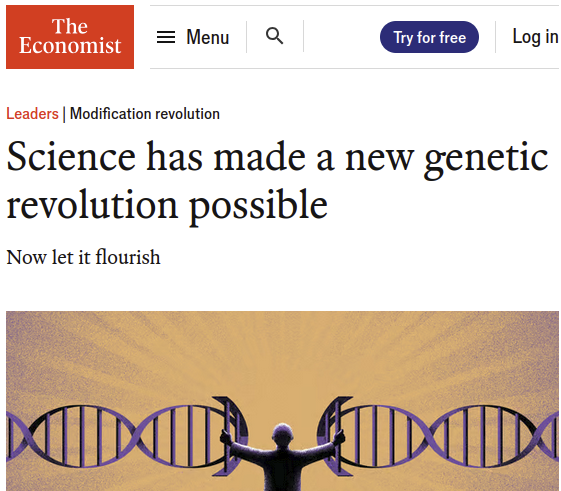
\includegraphics[width=\textwidth]{presentation-files/headlines/economist-2022-revolution.png}
        \end{subfigure}
        \hfill
        \begin{subfigure}[c]{0.45\textwidth}
            \vspace{0.25cm}

            \begin{colormixin}{15!bg}
            \textbf{Nature vs Nurture}
            \begin{enumerate}
                \item Genetics measure nature (initial endowment)
                \item Genes for social outcomes
                \item Deeper understanding of social outcomes, from genetics.
            \end{enumerate}
            \end{colormixin}
        \end{subfigure}
    \end{figure}
\end{frame}
%-------------------------------------------------------------------------------
\begin{frame}[noframenumbering]
    \frametitle{Introduction}
    \begin{beamercolorbox}{postit}
        \raggedright
        \vspace{0.01cm} \\
        ``\textbf{The difference of natural talents in different men}, is, in reality, much less than we are aware of [\ldots].
        The difference between the most dissimilar characters, between a philosopher and a common street porter, seems to arise \textbf{not so much from nature, as from habit, custom, and education}.''
        \hfill
        \underline{\textit{Adam Smith (1776), The Wealth of Nations, Volume 1 p. 16.}}
        \vspace{0.02cm}
    \end{beamercolorbox}
    \vspace{-0.25cm}
    \pause
    \begin{figure}[h!]
        \centering
        \singlespacing
        \begin{subfigure}[c]{0.5\textwidth}
            \centering
            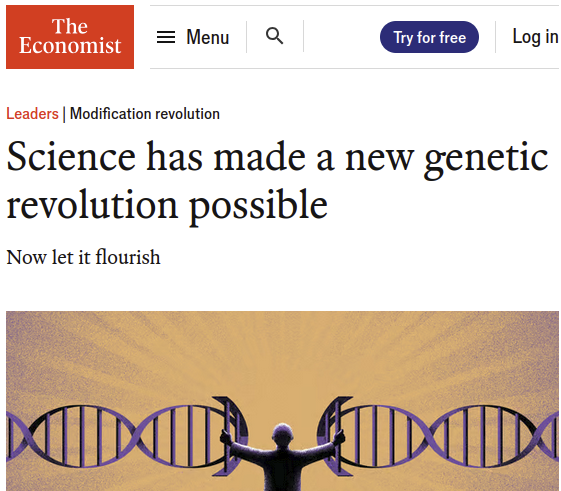
\includegraphics[width=\textwidth]{presentation-files/headlines/economist-2022-revolution.png}
        \end{subfigure}
        \hfill
        \begin{subfigure}[c]{0.45\textwidth}
            \textbf{Nature vs Nurture}
            \begin{enumerate}
                \item Genetics measure nature (initial endowment)
                \item Find genes associated with outcomes
                \item Deeper understanding of social outcomes, from genetics.
            \end{enumerate}
        \end{subfigure}
    \end{figure}
\end{frame}
%-------------------------------------------------------------------------------
\begin{frame}[noframenumbering]
    \frametitle{Introduction}
    \begin{beamercolorbox}{postit}
        \raggedright
        \vspace{0.01cm} \\
        ``\textbf{The difference of natural talents in different men}, is, in reality, much less than we are aware of [\ldots].
        The difference between the most dissimilar characters, between a philosopher and a common street porter, seems to arise \textbf{not so much from nature, as from habit, custom, and education}.''
        \hfill
        \underline{\textit{Adam Smith (1776), The Wealth of Nations, Volume 1 p. 16.}}
        \vspace{0.02cm}
    \end{beamercolorbox}
    \vspace{-0.25cm}
    \pause
    \begin{figure}[h!]
        \centering
        \singlespacing
        \begin{subfigure}[c]{0.4\textwidth}
            \vspace{-0.25cm}

            \textbf{Nature(?) vs Nurture}
            \begin{enumerate}
                \item Genetics measure one component of nature \\(at most\dots)
                \item Genes associated with outcomes are not the entire story
                \item Genetics gives new findings\pause, \textbf{with caveats.}
            \end{enumerate}
        \end{subfigure}
        \hfill
        \begin{subfigure}[c]{0.55\textwidth}
            \centering
            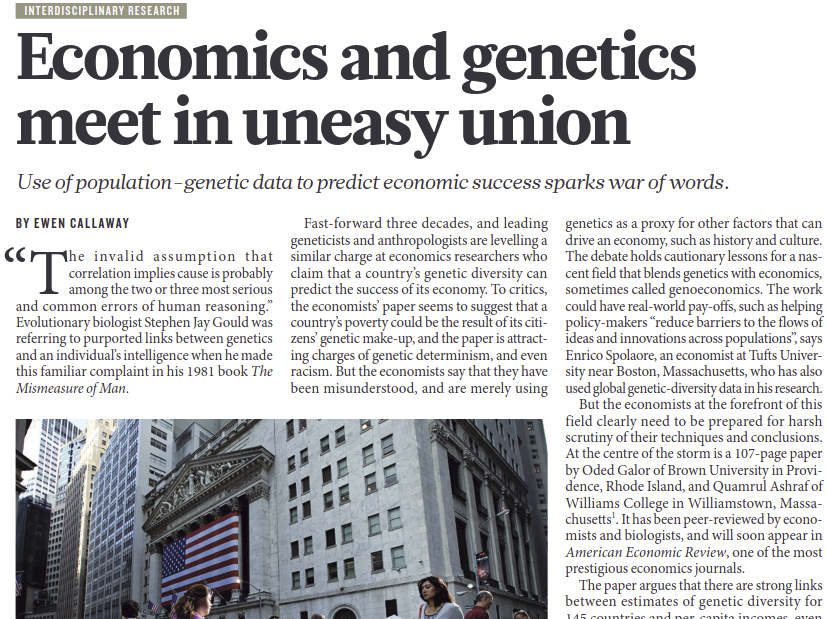
\includegraphics[width=\textwidth]{presentation-files/headlines/nature-2012-uneasy.png}
        \end{subfigure}
    \end{figure}
\end{frame}%-------------------------------------------------------------------------------
\begin{frame}[noframenumbering]
    \frametitle{Introduction}
    \textbf{How do genes associated with education affect labour outcomes?}
    \vspace{0.25cm}
    \begin{enumerate}
        \pause
        \item Causal design for random variation in a genetic measure for education.
        \begin{figure}
            \centering
            \singlespacing
            \vspace{-0.25cm}
            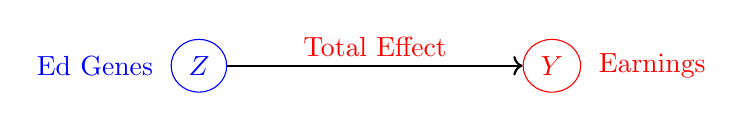
\begin{tikzpicture}
                \node[state,blue] (instrument) at (0,0) {$Z$};
                \node[state,red] (outcome) [right=3.75cm of instrument] {$Y$};
                \path[->, thick] (instrument) edge (outcome);
                % Label the nodes with econ examples
                \node[color=blue, left=0.1cm of instrument] {Ed Genes};
                \node[color=red, right=0.1cm of outcome] {Earnings};
                % Label the effect in the middle
                \path (instrument) -- (outcome) node[midway] (label) {};
                \node[color=red, above=-0.25cm of label] {Total Effect};
            \end{tikzpicture}
        \end{figure}
        \pause
        \item Decompose mechanisms by a mediation analysis (with an overlapping natural experiment).
        \begin{figure}
            \centering
            \singlespacing
            \vspace{-0.75cm}
            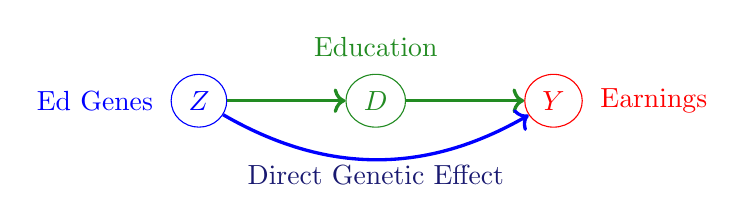
\begin{tikzpicture}
                \node[state,ForestGreen] (treatment) at (0,0) {$D$};
                \node[state,blue] (instrument) [left=1.5cm of treatment] {$Z$};
                \node[state,red] (outcome) [right=1.5cm of treatment] {$Y$};
                %\path[->] (instrument) edge (treatment);
                %\path[->] (treatment) edge (outcome);
                % Label the nodes with econ examples
                \node[color=blue, left=0.1cm of instrument] {Ed Genes};
                \node[color=red, right=0.1cm of outcome] {Earnings};
                \pause
                \node[color=ForestGreen, above=0.1cm of treatment] {Education};
                % Add in direct + indirect effects.
                %\path[->] (instrument) edge[bend right=45] (outcome);
                % Label the pathways with the colours
                \path[->, very thick, color=ForestGreen] (instrument) edge (treatment);
                \path[->, very thick, color=ForestGreen] (treatment) edge (outcome);
                \pause
                \path[->, very thick, color=blue] (instrument) edge[bend right=30] (outcome);
                \node[color=MidnightBlue, below=0.35cm of treatment] {Direct Genetic Effect};
            \end{tikzpicture}
        \end{figure}
        \pause
        \item Finding that genes associated with education do/not affect outcomes \textbf{directly or indirectly,} inferring they do/not measure intelligence, aptitude, or other factors.
    \end{enumerate}
\end{frame}%-------------------------------------------------------------------------------
\begin{frame}[noframenumbering]
    \frametitle{Introduction}
    \textbf{How do genes associated with education affect labour outcomes?}
    \vspace{0.25cm}
    \tableofcontents
\end{frame}
%-------------------------------------------------------------------------------
\section{1. Genetics \& Education}
%-------------------------------------------------------------------------------
\begin{frame}
    \frametitle{Genetics: a Primer}
    \begin{itemize}
        \item The human genome is a 3 billion-long sequence of base pairs
        \item $\approx 0.1\%$ these pairs differ between two average people
    \end{itemize}
    \begin{figure}
        \centering
        {\flushleft Person 1's DNA: \\}
        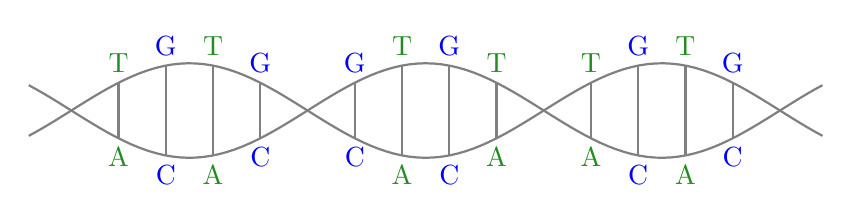
\begin{tikzpicture}
            % Draw the top DNA Helix
            \begin{scope}[scale=0.6, domain=-0.9:15.9, samples=101]
                % Draw the phosphate backbone.
                \draw[gray, thick] plot (\x,{sin(\x*36)});
                \draw[gray, thick] plot (\x,{-sin(\x*36)});
                % Draw the base pairs bonds
                \foreach \x in {0, 1, ...,14, 15}{
                    \draw[thick, gray] (\x,{-sin(\x*36)}) -- (\x,{sin(\x*36)});
                }
                % Label the base pairs.
                \foreach \x in {1, 3, 7, 9, 11, 13}{
                    \node[above, color=ForestGreen] at (\x,{abs(sin(\x*36))}) {T};
                    \node[below, color=ForestGreen] at (\x,{-abs(sin(\x*36))}) {A};
                }
                % Label the base pairs.
                \foreach \x in {2, 4, 6, 8, 12, 14}{
                    \node[above, color=blue] at (\x,{abs(sin(\x*36))}) {G};
                    \node[below, color=blue] at (\x,{-abs(sin(\x*36))}) {C};
                }
            \end{scope}
        \end{tikzpicture}
        \pause
        {\flushleft Person 2's DNA: \\}
        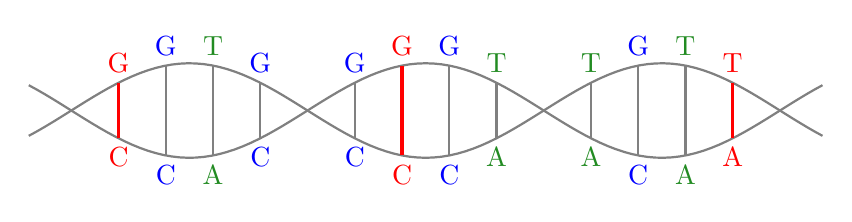
\begin{tikzpicture}
            % Draw the top DNA Helix
            \begin{scope}[scale=0.6, domain=-0.9:15.9, samples=101]
                % Draw the phosphate backbone.
                \draw[gray, thick] plot (\x,{sin(\x*36)});
                \draw[gray, thick] plot (\x,{-sin(\x*36)});
                % Draw the base pairs bonds
                \foreach \x in {0, 1, ..., 15}{
                    \draw[thick, gray] (\x,{-sin(\x*36)}) -- (\x,{sin(\x*36)});
                }
                % Label the base pairs.
                \foreach \x in {3, 9, 11, 13}{
                    \node[above, color=ForestGreen] at (\x,{abs(sin(\x*36))}) {T};
                    \node[below, color=ForestGreen] at (\x,{-abs(sin(\x*36))}) {A};
                }
                % Label the base pairs.
                \foreach \x in {2, 4, 6, 8, 12}{
                    \node[above, color=blue] at (\x,{abs(sin(\x*36))}) {G};
                    \node[below, color=blue] at (\x,{-abs(sin(\x*36))}) {C};
                }
                % Difference in the base pairs.
                \foreach \x in {1, 7, 14}{
                    \draw[very thick, red] (\x,{-sin(\x*36)}) -- (\x,{sin(\x*36)});
                }
                \node[above, color=red] at (1, { abs(sin(1 *36))}) {G};
                \node[below, color=red] at (1, {-abs(sin(1 *36))}) {C};
                \node[above, color=red] at (7, { abs(sin(7 *36))}) {G};
                \node[below, color=red] at (7, {-abs(sin(7 *36))}) {C};
                \node[above, color=red] at (14,{ abs(sin(14*36))}) {T};
                \node[below, color=red] at (14,{-abs(sin(14*36))}) {A};
            \end{scope}
        \end{tikzpicture}
    \end{figure}
\end{frame}
%-------------------------------------------------------------------------------
\begin{frame}[noframenumbering]
    \frametitle{Genetics: a Primer}
    \begin{itemize}
        \item The human genome is a 3 billion-long sequence of base pairs
        \item $\approx 0.1\%$ these pairs differ between two average people
    \end{itemize}
    \begin{figure}
        \centering
        {\flushleft Person 1's DNA: \\}
        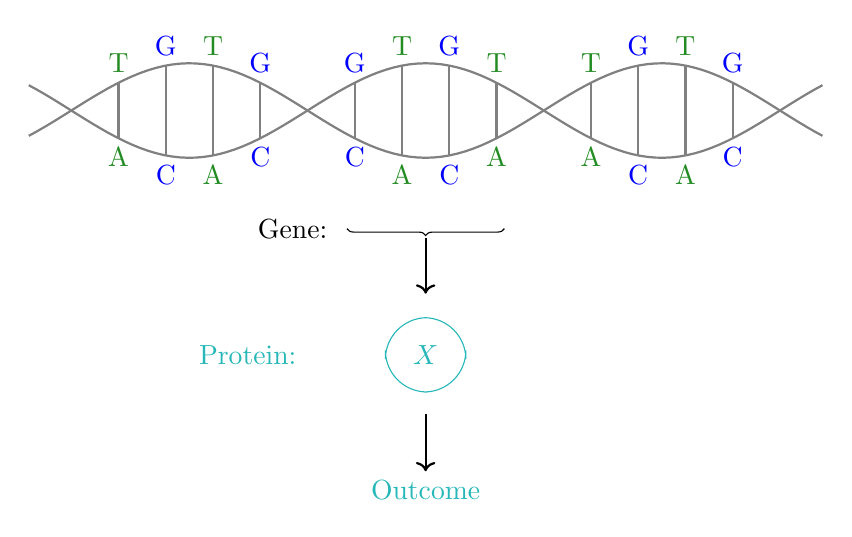
\begin{tikzpicture}[
            box/.style = {draw,inner sep=10pt,rounded corners=15pt}]
            % Draw the top DNA Helix
            \begin{scope}[scale=0.6, domain=-0.9:15.9, samples=101]
                % Draw the phosphate backbone.
                \draw[gray, thick] plot (\x,{sin(\x*36)});
                \draw[gray, thick] plot (\x,{-sin(\x*36)});
                % Draw the base pairs bonds
                \foreach \x in {0, 1, ...,14, 15}{
                    \draw[thick, gray] (\x,{-sin(\x*36)}) -- (\x,{sin(\x*36)});
                }
                % Label the base pairs.
                \foreach \x in {1, 3, 7, 9, 11, 13}{
                    \node[above, color=ForestGreen] at (\x,{abs(sin(\x*36))}) {T};
                    \node[below, color=ForestGreen] at (\x,{-abs(sin(\x*36))}) {A};
                }
                % Label the base pairs.
                \foreach \x in {2, 4, 6, 8, 12, 14}{
                    \node[above, color=blue] at (\x,{abs(sin(\x*36))}) {G};
                    \node[below, color=blue] at (\x,{-abs(sin(\x*36))}) {C};
                }
            \end{scope}
            % Identify the gene region
            \draw[decorate, decoration = {brace}] (5.5,-1.5) -- (3.5,-1.5);
            \node (gene) at (4.5,-1.5) {};
            \node[left=of gene] {Gene:};
            % Show that the gene leads to a protein
            \pause
            \node[box,color=BlueGreen, below=of gene] (protein) {$X$};
            \node[color=BlueGreen, left=of protein] {Protein:};
            \node[above=0.05cm of protein] (proteinabove) {};
            \draw[->,thick] (gene) -- (proteinabove);
            % Show that the protein leads to outcome.
            \node[color=BlueGreen, below=of protein] (outcome) {Outcome};
            \node[below=0.025cm of protein] (proteinbelow) {};
            \draw[->,thick] (proteinbelow) -- (outcome);
        \end{tikzpicture}
    \end{figure}
\end{frame}
%-------------------------------------------------------------------------------
\begin{frame}[noframenumbering]
    \frametitle{Genetics: a Primer}
    \begin{itemize}
        \item The human genome is a 3 billion-long sequence of base pairs
        \item $\approx 0.1\%$ these \textcolor{red}{pairs differ} between two average people
    \end{itemize}
    \begin{figure}
        \centering
        {\flushleft Person 2's DNA: \\}
        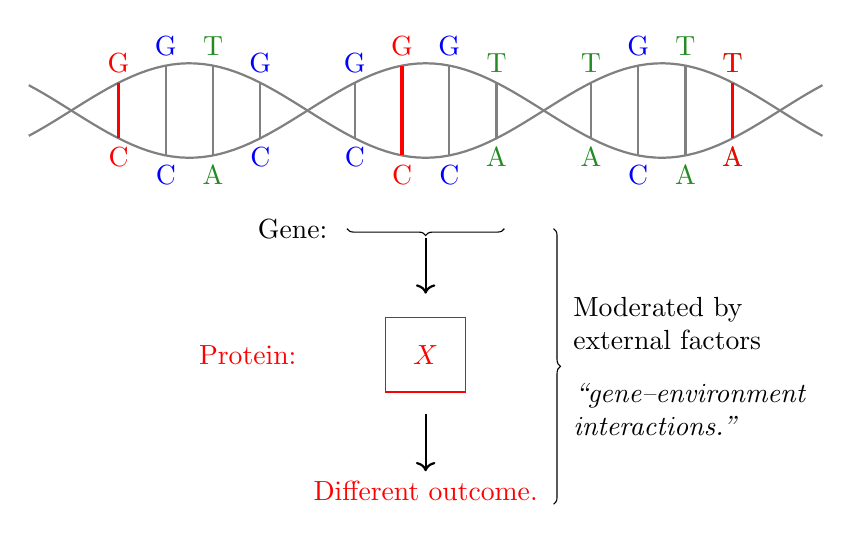
\begin{tikzpicture}[
            box/.style = {draw,inner sep=10pt,rounded corners=0pt}]
            % Draw the top DNA Helix
            \begin{scope}[scale=0.6, domain=-0.9:15.9, samples=101]
                % Draw the phosphate backbone.
                \draw[gray, thick] plot (\x,{sin(\x*36)});
                \draw[gray, thick] plot (\x,{-sin(\x*36)});
                % Draw the base pairs bonds
                \foreach \x in {0, 1, ...,14, 15}{
                    \draw[thick, gray] (\x,{-sin(\x*36)}) -- (\x,{sin(\x*36)});
                }
                % Label the base pairs.
                \foreach \x in {3, 9, 11, 13, 14}{
                    \node[above, color=ForestGreen] at (\x,{abs(sin(\x*36))}) {T};
                    \node[below, color=ForestGreen] at (\x,{-abs(sin(\x*36))}) {A};
                }
                % Label the base pairs.
                \foreach \x in {2, 4, 6, 8, 12}{
                    \node[above, color=blue] at (\x,{abs(sin(\x*36))}) {G};
                    \node[below, color=blue] at (\x,{-abs(sin(\x*36))}) {C};
                }
                %\pause
                % Difference in the base pairs.
                \foreach \x in {1, 7, 14}{
                    \draw[very thick, red] (\x,{-sin(\x*36)}) -- (\x,{sin(\x*36)});
                }
                \node[above, color=red] at (1, { abs(sin(1 *36))}) {G};
                \node[below, color=red] at (1, {-abs(sin(1 *36))}) {C};
                \node[above, color=red] at (7, { abs(sin(7 *36))}) {G};
                \node[below, color=red] at (7, {-abs(sin(7 *36))}) {C};
                \node[above, color=red] at (14,{ abs(sin(14*36))}) {T};
                \node[below, color=red] at (14,{-abs(sin(14*36))}) {A};
            \end{scope}
            % Identify the gene region
            \pause
            \draw[decorate, decoration = {brace}] (5.5,-1.5) -- (3.5,-1.5);
            \node (gene) at (4.5,-1.5) {};
            \node[left=of gene] {Gene:};
            % Show that the gene leads to a protein
            \node[box,color=red, below=of gene] (protein) {$X$};
            \node[color=red, left=of protein] {Protein:};
            \node[above=0.05cm of protein] (proteinabove) {};
            \draw[->,thick] (gene) -- (proteinabove);
            % Show that the protein leads to outcome.
            \node[color=red,below=of protein] (outcome) {Different outcome.};
            \node[below=0.025cm of protein] (proteinbelow) {};
            \draw[->,thick] (proteinbelow) -- (outcome);
            % Add on a part referencing environment interactions
            \pause
            \draw[decorate, decoration = {brace}] (6.125,-1.5) -- (6.125,-5);
            \node[text width=3cm] (environment) at (7.875,-3.25) {
                Moderated by \\ external factors \\ \vspace{0.25cm}
                    \textit{``gene--environment \\interactions.''}};
        \end{tikzpicture}
    \end{figure}
\end{frame}
%-------------------------------------------------------------------------------
\begin{frame}
    \frametitle{Polygenic Index \& Education (Ed PGI)}
    \vspace{-0.25cm}

    \begin{figure}
        \centering
        \makebox[\textwidth][c]{
            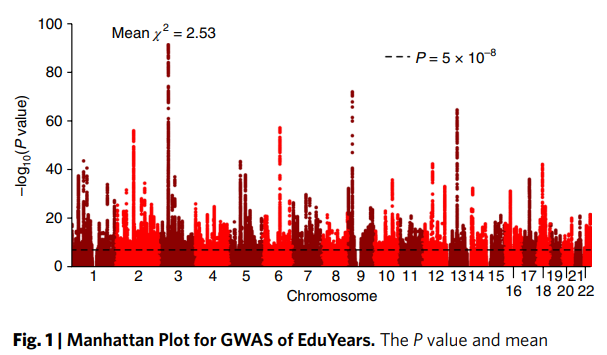
\includegraphics[width=0.75\textwidth]{
                presentation-files/okbay-2018.png}}
    \end{figure}
    \begin{beamercolorbox}{postit}
        \small
        \vspace{0.01cm}
        
        \raggedright
        ``A large-scale genetic association analysis of educational attainment in a sample of approximately 1.1 million individuals and identify \textbf{1,271 independent genome-wide-significant SNPs...
        generating a Polygenic Index} that explains 11--13\% of the variance in educational attainment and 7--10\% of the variance in cognitive performance.''
        \hfill
        \underline{\textit{Abstract --- Lee et al. (2018, Nature Genetics)}}
        \vspace{0.025cm}
    \end{beamercolorbox}
\end{frame}
%-------------------------------------------------------------------------------
\begin{frame}[noframenumbering]
    \frametitle{Polygenic Index \& Education (Ed PGI)}
    \begin{figure}
        \centering
        {\flushleft Person 1's DNA: \\}
        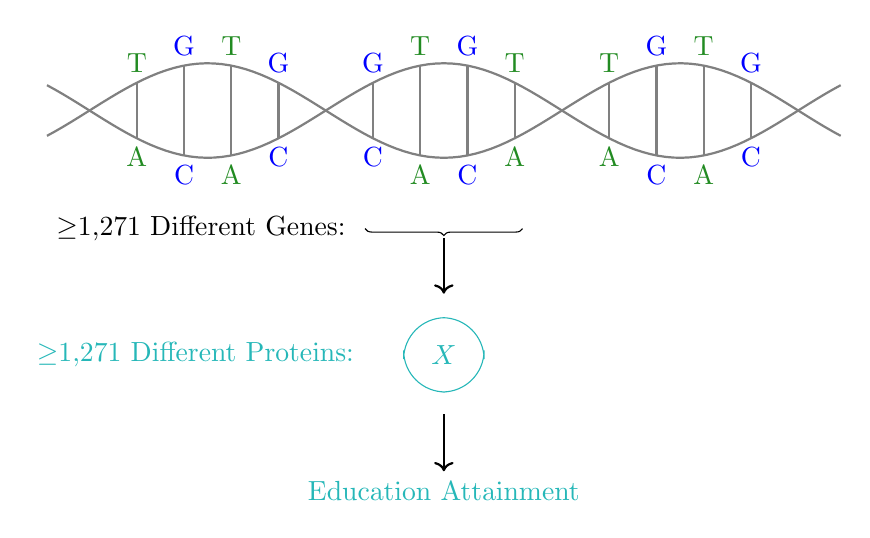
\begin{tikzpicture}[
            box/.style = {draw,inner sep=10pt,rounded corners=15pt}]
            % Draw the top DNA Helix
            \begin{scope}[scale=0.6, domain=-0.9:15.9, samples=101]
                % Draw the phosphate backbone.
                \draw[gray, thick] plot (\x,{sin(\x*36)});
                \draw[gray, thick] plot (\x,{-sin(\x*36)});
                % Draw the base pairs bonds
                \foreach \x in {0, 1, ...,14, 15}{
                    \draw[thick, gray] (\x,{-sin(\x*36)}) -- (\x,{sin(\x*36)});
                }
                % Label the base pairs.
                \foreach \x in {1, 3, 7, 9, 11, 13}{
                    \node[above, color=ForestGreen] at (\x,{abs(sin(\x*36))}) {T};
                    \node[below, color=ForestGreen] at (\x,{-abs(sin(\x*36))}) {A};
                }
                % Label the base pairs.
                \foreach \x in {2, 4, 6, 8, 12, 14}{
                    \node[above, color=blue] at (\x,{abs(sin(\x*36))}) {G};
                    \node[below, color=blue] at (\x,{-abs(sin(\x*36))}) {C};
                }
            \end{scope}
            % Identify the gene region
            \draw[decorate, decoration = {brace}] (5.5,-1.5) -- (3.5,-1.5);
            \node (gene) at (4.5,-1.5) {};
            \node[left=of gene] {$\geq$1,271 Different Genes:};
            % Show that the gene leads to a protein
            \node[box,color=BlueGreen, below=of gene] (protein) {$X$};
            \node[color=BlueGreen, left=0.5cm of protein] {$\geq$1,271 Different Proteins:};
            \node[above=0.05cm of protein] (proteinabove) {};
            \draw[->,thick] (gene) -- (proteinabove);
            % Show that the protein leads to outcome.
            \node[color=BlueGreen,below=of protein] (outcome) {
                Education Attainment};
            \node[below=0.025cm of protein] (proteinbelow) {};
            \draw[->,thick] (proteinbelow) -- (outcome);
        \end{tikzpicture}
    \end{figure}
    \vspace{1cm}
\end{frame}
%-------------------------------------------------------------------------------
\begin{frame}[noframenumbering]
    \frametitle{Polygenic Index \& Education (Ed PGI)}
    \begin{figure}
        \centering
        {\flushleft Person 2's DNA: \\}
        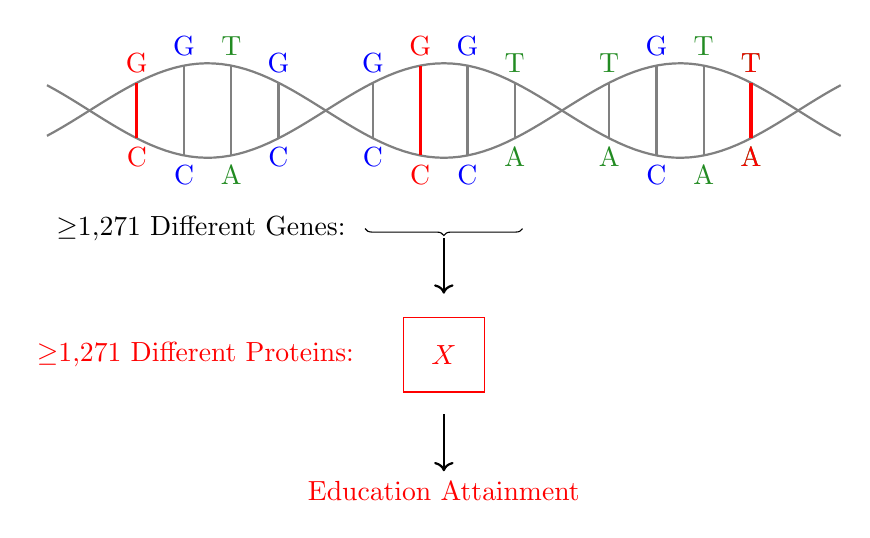
\begin{tikzpicture}[
            box/.style = {draw,inner sep=10pt,rounded corners=0pt}]
            % Draw the top DNA Helix
            \begin{scope}[scale=0.6, domain=-0.9:15.9, samples=101]
                % Draw the phosphate backbone.
                \draw[gray, thick] plot (\x,{sin(\x*36)});
                \draw[gray, thick] plot (\x,{-sin(\x*36)});
                % Draw the base pairs bonds
                \foreach \x in {0, 1, ...,14, 15}{
                    \draw[thick, gray] (\x,{-sin(\x*36)}) -- (\x,{sin(\x*36)});
                }
                % Label the base pairs.
                \foreach \x in {3, 9, 11, 13, 14}{
                    \node[above, color=ForestGreen] at (\x,{abs(sin(\x*36))}) {T};
                    \node[below, color=ForestGreen] at (\x,{-abs(sin(\x*36))}) {A};
                }
                % Label the base pairs.
                \foreach \x in {2, 4, 6, 8, 12}{
                    \node[above, color=blue] at (\x,{abs(sin(\x*36))}) {G};
                    \node[below, color=blue] at (\x,{-abs(sin(\x*36))}) {C};
                }
                % Difference in the base pairs.
                \foreach \x in {1, 7, 14}{
                    \draw[very thick, red] (\x,{-sin(\x*36)}) -- (\x,{sin(\x*36)});
                }
                \node[above, color=red] at (1, { abs(sin(1 *36))}) {G};
                \node[below, color=red] at (1, {-abs(sin(1 *36))}) {C};
                \node[above, color=red] at (7, { abs(sin(7 *36))}) {G};
                \node[below, color=red] at (7, {-abs(sin(7 *36))}) {C};
                \node[above, color=red] at (14,{ abs(sin(14*36))}) {T};
                \node[below, color=red] at (14,{-abs(sin(14*36))}) {A};
            \end{scope}
            % Identify the gene region
            \draw[decorate, decoration = {brace}] (5.5,-1.5) -- (3.5,-1.5);
            \node (gene) at (4.5,-1.5) {};
            \node[left=of gene] {$\geq$1,271 Different Genes:};
            % Show that the gene leads to a protein
            \node[box,color=red, below=of gene] (protein) {$X$};
            \node[color=red, left=0.5cm of protein] {$\geq$1,271 Different Proteins:};
            \node[above=0.05cm of protein] (proteinabove) {};
            \draw[->,thick] (gene) -- (proteinabove);
            % Show that the protein leads to outcome.
            \node[color=red,below=of protein] (outcome) {
                Education Attainment};
            \node[below=0.025cm of protein] (proteinbelow) {};
            \draw[->,thick] (proteinbelow) -- (outcome);
        \end{tikzpicture}
    \end{figure}
    \pause
    \begin{itemize}
        \item In practice, we do not know exact location of relevant gene regions
        \item Nor the associated protein $+$ what they do
    \end{itemize}
\end{frame}
%-------------------------------------------------------------------------------
\begin{frame}[noframenumbering]
    \frametitle{Polygenic Index \& Education (Ed PGI)}
    \begin{figure}
        \centering
        {\flushleft Person 2's DNA: \\}
        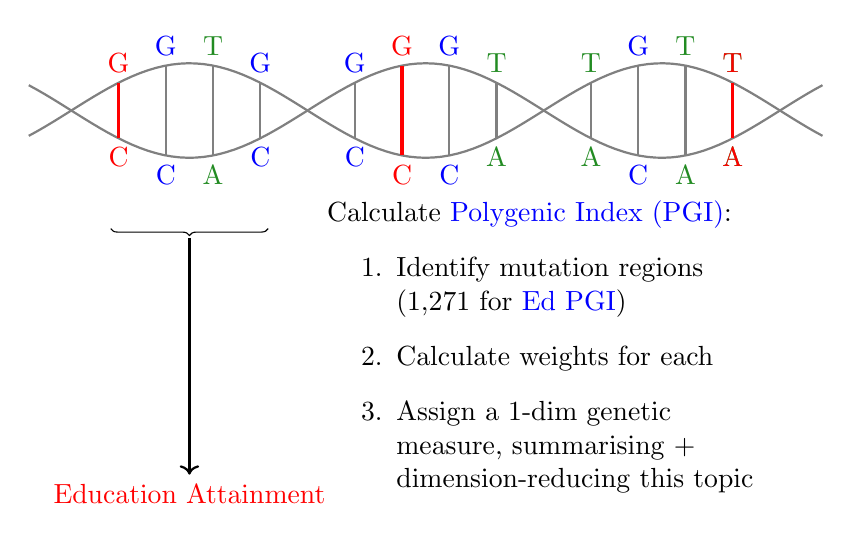
\begin{tikzpicture}[
            box/.style = {draw,inner sep=10pt,rounded corners=15pt}]
            % Draw the top DNA Helix
            \begin{scope}[scale=0.6, domain=-0.9:15.9, samples=101]
                % Draw the phosphate backbone.
                \draw[gray, thick] plot (\x,{sin(\x*36)});
                \draw[gray, thick] plot (\x,{-sin(\x*36)});
                % Draw the base pairs bonds
                \foreach \x in {0, 1, ...,14, 15}{
                    \draw[thick, gray] (\x,{-sin(\x*36)}) -- (\x,{sin(\x*36)});
                }
                % Label the base pairs.
                \foreach \x in {3, 9, 11, 13, 14}{
                    \node[above, color=ForestGreen] at (\x,{abs(sin(\x*36))}) {T};
                    \node[below, color=ForestGreen] at (\x,{-abs(sin(\x*36))}) {A};
                }
                % Label the base pairs.
                \foreach \x in {2, 4, 6, 8, 12}{
                    \node[above, color=blue] at (\x,{abs(sin(\x*36))}) {G};
                    \node[below, color=blue] at (\x,{-abs(sin(\x*36))}) {C};
                }
                % Difference in the base pairs.
                \foreach \x in {1, 7, 14}{
                    \draw[very thick, red] (\x,{-sin(\x*36)}) -- (\x,{sin(\x*36)});
                }
                \node[above, color=red] at (1, { abs(sin(1 *36))}) {G};
                \node[below, color=red] at (1, {-abs(sin(1 *36))}) {C};
                \node[above, color=red] at (7, { abs(sin(7 *36))}) {G};
                \node[below, color=red] at (7, {-abs(sin(7 *36))}) {C};
                \node[above, color=red] at (14,{ abs(sin(14*36))}) {T};
                \node[below, color=red] at (14,{-abs(sin(14*36))}) {A};
            \end{scope}
            % Identify the gene region
            \draw[decorate, decoration = {brace}] (2.5,-1.5) -- (0.5,-1.5);
            \node (gene) at (1.5,-1.5) {};
            % Show that the gene leads to an outcome
            \node[color=red, below=3.0cm of gene] (outcome) {
                Education Attainment};
            \draw[->,thick] (gene) -- (outcome);
            % Show the PGI Process
            \pause
            \node[text width=5.5cm] at (6,-3) {
                Calculate \textcolor{blue}{Polygenic Index (PGI)}:
                \begin{enumerate}
                    \item Identify mutation regions (1,271 for \textcolor{blue}{Ed PGI})
                    \item Calculate weights for each
                    \item Assign a 1-dim genetic measure, summarising $+$ dimension-reducing this topic
                \end{enumerate}};
        \end{tikzpicture}
    \end{figure}
    \begin{itemize}
        \item In practice, we do not know exact location of relevant gene regions
        \item Nor the associated protein $+$ what they do
    \end{itemize}
\end{frame}
%-------------------------------------------------------------------------------
\begin{frame}[noframenumbering]
    \frametitle{Polygenic Index \& Education (Ed PGI)}
    \begin{beamercolorbox}{postit}
        \small
        \vspace{0.025cm}
        
        \raggedright
        ``A large-scale genetic association analysis of educational attainment in a sample of approximately 1.1 million individuals and identify \textbf{1,271 independent genome-wide-significant SNPs...
        generating a Polygenic Index} that explains 11--13\% of the variance in educational attainment and 7--10\% of the variance in cognitive performance.''
        \hfill
        \underline{\textit{Abstract --- Lee et al. (2018, Nature Genetics)}}
        \vspace{0.025cm}
    \end{beamercolorbox}
    \begin{figure}
        \centering
        \makebox[\textwidth][c]{
            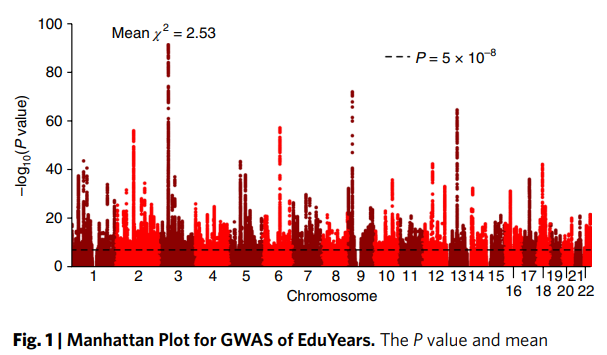
\includegraphics[width=0.75\textwidth]{
                presentation-files/okbay-2018.png}}
    \end{figure}
\end{frame}
%-------------------------------------------------------------------------------
\begin{frame}
    \frametitle{Polygenic Index \& Education (Ed PGI)}
    \textbf{Education Polygenic Index (Ed PGI):} \\
    A weighted sum of single letter gene changes predicting years of education.
    \begin{figure}
        \centering
        {\flushleft Person 1's DNA: \\}
        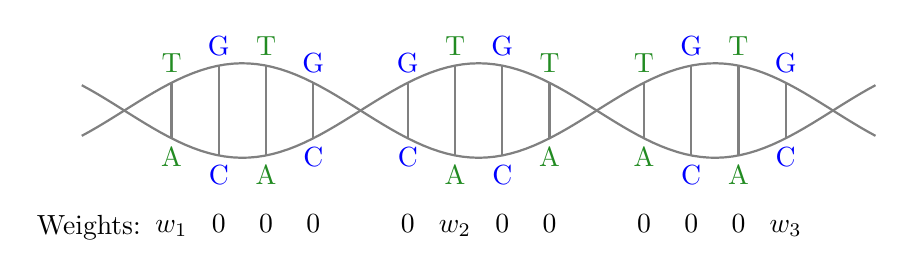
\begin{tikzpicture}
            % Draw the top DNA Helix
            \begin{scope}[scale=0.6, domain=-0.9:15.9, samples=101]
                % Draw the phosphate backbone.
                \draw[gray, thick] plot (\x,{sin(\x*36)});
                \draw[gray, thick] plot (\x,{-sin(\x*36)});
                % Draw the base pairs bonds
                \foreach \x in {0, 1, ...,14, 15}{
                    \draw[thick, gray] (\x,{-sin(\x*36)}) -- (\x,{sin(\x*36)});
                }
                % Label the base pairs.
                \foreach \x in {1, 3, 7, 9, 11, 13}{
                    \node[above, color=ForestGreen] at (\x,{abs(sin(\x*36))}) {T};
                    \node[below, color=ForestGreen] at (\x,{-abs(sin(\x*36))}) {A};
                }
                % Label the base pairs.
                \foreach \x in {2, 4, 6, 8, 12, 14}{
                    \node[above, color=blue] at (\x,{abs(sin(\x*36))}) {G};
                    \node[below, color=blue] at (\x,{-abs(sin(\x*36))}) {C};
                }
                % Annotate with weights
                \node[below] at (-0.75,-2) {Weights:};
                \foreach \x in {2, 3, 4, 6, 8, 9, 11, 12, 13}{
                    \node[below] at (\x,-2) {0};
                }
                \node[below] at (1, -2.125) {$w_1$};
                \node[below] at (7, -2.125) {$w_2$};
                \node[below] at (14,-2.125) {$w_3$};
            \end{scope}
        \end{tikzpicture}
    \end{figure}
    \pause
    \vfill
    Person 1's Ed PGI:
    \[ Z = \sum_{j \in J} w_j
        \textcolor{red}{\indicator{\text{one-letter change at $j$}}}
        = 0 \]
    \textcolor{white}{
        \textbf{Note:} Humans have two copies of each chromosome, so indicator is 0, 1, 2 corresponding to how many copies one has.}
\end{frame}
%-------------------------------------------------------------------------------
\begin{frame}[noframenumbering]
    \frametitle{Polygenic Index \& Education (Ed PGI)}
    \textbf{Education Polygenic Index (Ed PGI):} \\
    A weighted sum of single letter gene changes predicting years of education.
    \begin{figure}
        \centering
        {\flushleft Person 2's DNA: \\}
        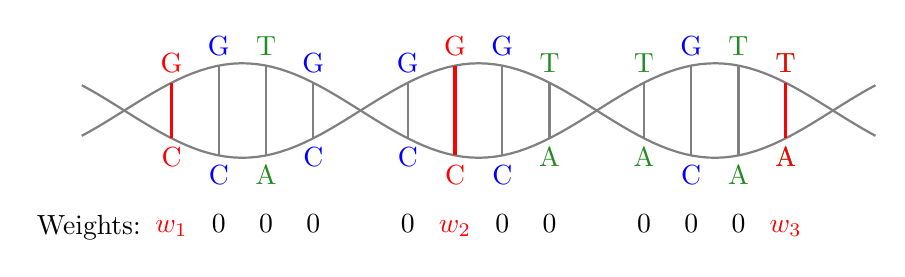
\begin{tikzpicture}
            % Draw the top DNA Helix
            \begin{scope}[scale=0.6, domain=-0.9:15.9, samples=101]
                % Draw the phosphate backbone.
                \draw[gray, thick] plot (\x,{sin(\x*36)});
                \draw[gray, thick] plot (\x,{-sin(\x*36)});
                % Draw the base pairs bonds
                \foreach \x in {0, 1, ...,14, 15}{
                    \draw[thick, gray] (\x,{-sin(\x*36)}) -- (\x,{sin(\x*36)});
                }
                % Label the base pairs.
                \foreach \x in {3, 9, 11, 13, 14}{
                    \node[above, color=ForestGreen] at (\x,{abs(sin(\x*36))}) {T};
                    \node[below, color=ForestGreen] at (\x,{-abs(sin(\x*36))}) {A};
                }
                % Label the base pairs.
                \foreach \x in {2, 4, 6, 8, 12}{
                    \node[above, color=blue] at (\x,{abs(sin(\x*36))}) {G};
                    \node[below, color=blue] at (\x,{-abs(sin(\x*36))}) {C};
                }
                % Difference in the base pairs.
                \foreach \x in {1, 7, 14}{
                    \draw[very thick, red] (\x,{-sin(\x*36)}) -- (\x,{sin(\x*36)});
                }
                \node[above, color=red] at (1, { abs(sin(1*36))})  {G};
                \node[below, color=red] at (1, {-abs(sin(1*36))})  {C};
                \node[above, color=red] at (7, { abs(sin(7*36))})  {G};
                \node[below, color=red] at (7, {-abs(sin(7*36))})  {C};
                \node[above, color=red] at (14,{ abs(sin(14*36))}) {T};
                \node[below, color=red] at (14,{-abs(sin(14*36))}) {A};
                % Annotate with weights
                \node[below] at (-0.75,-2) {Weights:};
                \foreach \x in {2, 3, 4, 6, 8, 9, 11, 12, 13}{
                    \node[below] at (\x,-2) {0};
                }
                \node[below, color=red] at (1, -2.125) {\textcolor{red}{$w_1$}};
                \node[below, color=red] at (7, -2.125) {\textcolor{red}{$w_2$}};
                \node[below, color=red] at (14,-2.125) {\textcolor{red}{$w_3$}};
            \end{scope}
        \end{tikzpicture}
    \end{figure}
    \vfill
    Person 2's Ed PGI:
    \[ Z = \sum_{j \in J}
        \textcolor{red}{w_j} \indicator{\text{one-letter change at $j$}}
    =   \textcolor{red}{w_1} +
        \textcolor{red}{w_2} +
        \textcolor{red}{w_3} \]
    \pause
    \textbf{Note:} Humans have two copies of each chromosome, so indicator is 0, 1, 2 corresponding to how many copies one has.
\end{frame}
%-------------------------------------------------------------------------------
\begin{frame}
    \frametitle{Education Polygenic Index (Ed PGI)}
    Previous economics $+$ science research shows Ed PGI is strongly associated with multiple labour market outcomes:
    \vspace{0.25cm}

    % Define counter for table.
    \newcounter{rownum}
    \setcounter{rownum}{0}
    \newcommand{\rownum}{\stepcounter{rownum}
        \textbf{\textcolor{blue}{\arabic{rownum}. \;\;}} }
    \begin{tabular}{>{\rownum}l p{6cm}}
        Retirement wealth              & (Barth et al., 2020) \\
        Life-cycle income              & (Barth et al., 2022) \\
        Longevity                      & (Marioni et al., 2016) \\
        Primary school performance     & (Aagaard-Houmark et al., 2022) \\
        Parental--child care (nurture) & (Aagaard-Houmark et al., 2024) \\
            %\newline (Muslimova et al. 2024) \\
        Socioeconomic Status           & (Carvalho, 2024) \\
        $\hdots$                       &  \\
        Many in-progress               & (Forthcoming)  
    \end{tabular}

    \vspace{0.5cm}
    \textbf{Open question:} What are the mechanisms behind Ed PGI's effects?
    \begin{itemize}
        \item Is education the \textbf{only way} it is related to outcomes?
        \item Is there a \textbf{direct genetic relationship}, absent returns to education? 
    \end{itemize}
\end{frame}
%-------------------------------------------------------------------------------
\begin{frame}[noframenumbering]
    \frametitle{Education Polygenic Index (Ed PGI)}
    \vspace{-0.5cm}
    \begin{figure}
        \centering
        \singlespacing
        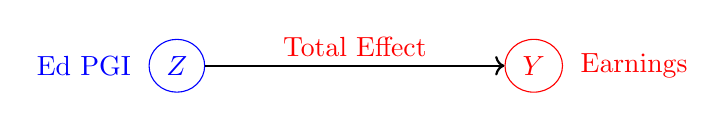
\begin{tikzpicture}
            \node[state,blue] (instrument) at (0,0) {$Z$};
            \node[state,red] (outcome) [right=3.8cm of instrument] {$Y$};
            \path[->, thick] (instrument) edge (outcome);
            % Label the nodes with econ examples
            \node[color=blue, left=0.1cm of instrument] {Ed PGI};
            \node[color=red, right=0.1cm of outcome] {Earnings};
            % Label the effect in the middle
            \path (instrument) -- (outcome) node[midway] (label) {};
            \node[color=red, above=-0.25cm of label] {Total Effect};
        \end{tikzpicture}
    \end{figure}
    I look at how Ed PGI \textbf{causally affects} labour market earnings,
    \pause and \textbf{model how much this relationship is because of the education channel.}
    \begin{figure}
        \centering
        \singlespacing
        \vspace{-0.5cm}
        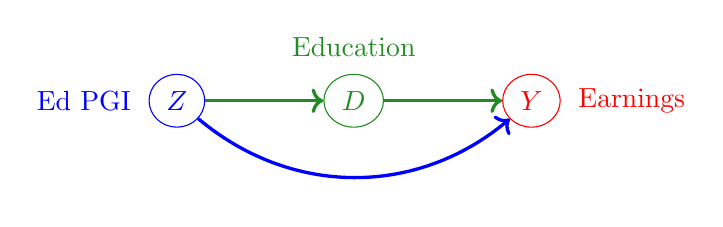
\begin{tikzpicture}
            \node[state,ForestGreen] (treatment) at (0,0) {$D$};
            \node[state,blue] (instrument) [left=1.5cm of treatment] {$Z$};
            \node[state,red] (outcome) [right=1.5cm of treatment] {$Y$};
            %\path[->] (instrument) edge (treatment);
            %\path[->] (treatment) edge (outcome);
            % Label the nodes with econ examples
            \node[color=blue, left=0.1cm of instrument] {Ed PGI};
            \node[color=red, right=0.1cm of outcome] {Earnings};
            \node[color=ForestGreen, above=0.1cm of treatment] {Education};
            % Add in direct effects.
            %\path[->] (instrument) edge[bend right=45] (outcome);
            % Label the pathways with the colours
            \path[->, very thick, color=ForestGreen] (instrument) edge (treatment);
            \path[->, very thick, color=ForestGreen] (treatment) edge (outcome);
            \path[->, very thick, color=blue] (instrument) edge[bend right=40] (outcome);
        \end{tikzpicture}
    \end{figure}
    \vspace{-0.5cm}
    \begin{table}
        \centering
        \begin{tabular}{c c c c c}
            \textcolor{red}{Total Effect} & $=$ &
            \textcolor{ForestGreen}{Indirect Effect} & $+$ &
            \textcolor{blue}{Direct Effect} \\
            \textcolor{red}{(Ed PGI $\to$ Earnings)}
            \pause
            && \textcolor{ForestGreen}{(Education)}
            \pause
            && \textcolor{blue}{(Genetic)}
        \end{tabular}
    \end{table}
    \pause
    \textbf{Contributions:}
    \begin{itemize}
        \item Connect new genetic measures to classic labour econ topics
        \item Mediation methods in a natural experiment setting
        \item \textbf{Test:} \textit{``Genetic measures correlated with education affect earnings \textbf{beyond just education}'' --- Barth Papageorge Thom (2020).}
    \end{itemize}
\end{frame}
%-------------------------------------------------------------------------------
\subsection{Data: \sout{UK Biobank} Health \& Retirement Study (HRS)}
%-------------------------------------------------------------------------------
\begin{frame}
    \frametitle{Data: UKBiobank}
    A dd in slide here describing UK Biobank, large sample size, etc.
    \vfill
    Access has not been processed yet, so I am merely describing the research design here.
    And some correlational evidence with (public) HRS data. 
\end{frame}
%-------------------------------------------------------------------------------
\begin{frame}
    \frametitle{Data: \sout{UK Biobank} Health \& Retirement Study (HRS)}
    A representative panel of retirement-age Americans 1990--2021.
    \vspace{-0.5cm}

    \begin{figure}
        \centering
        \singlespacing
        %\caption{Distribution of HRS Education Measures.}
        \begin{subfigure}[b]{0.495\textwidth}
            \centering
            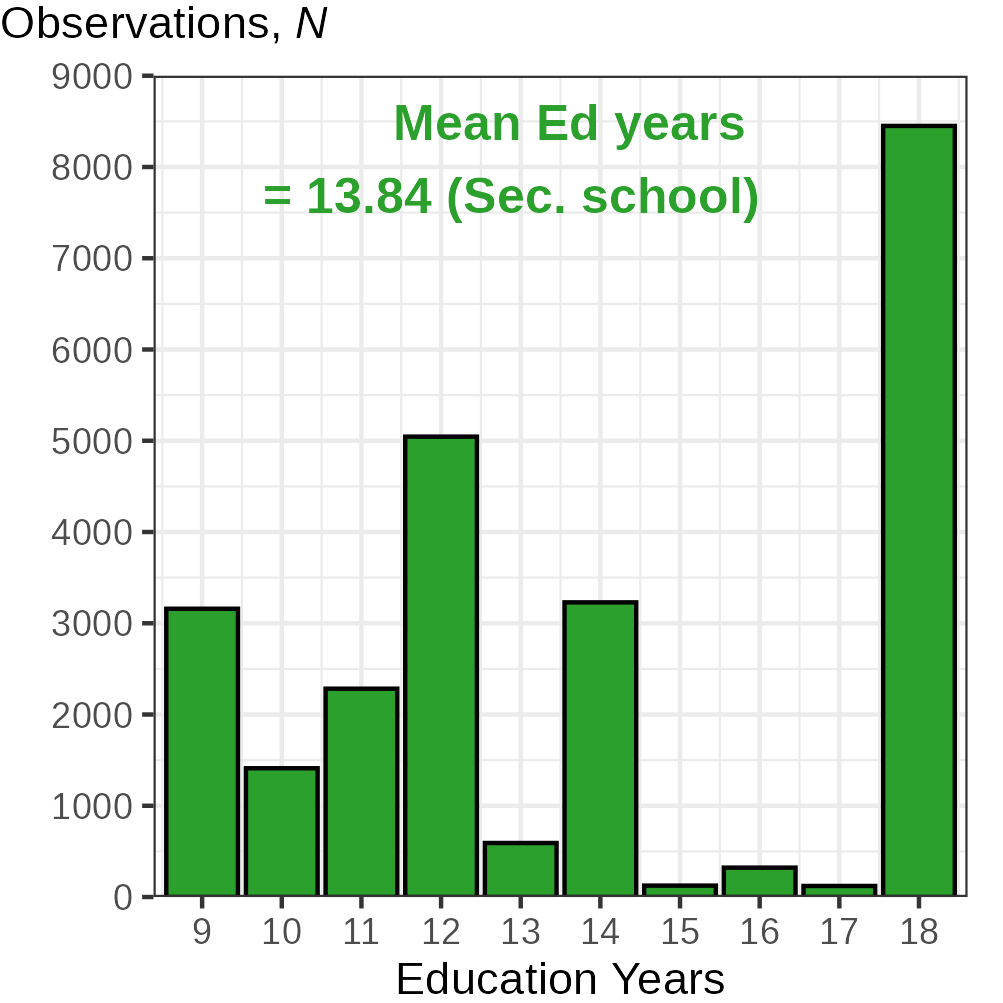
\includegraphics[width=\textwidth]{../text/sections/figures/edyears-hist.png}
            \label{fig:edyears-hist}
        \end{subfigure}
        \begin{subfigure}[b]{0.495\textwidth}
            \centering
            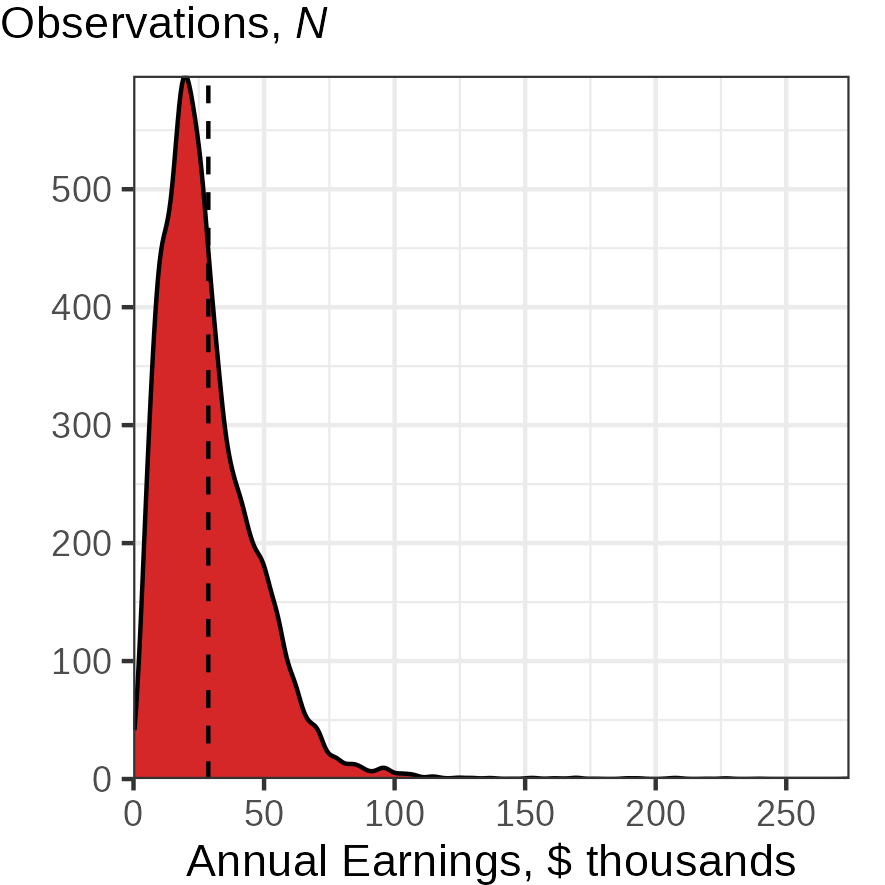
\includegraphics[width=\textwidth]{../text/sections/figures/earnings-hist.png}
            \label{fig:earnings-hist}
        \end{subfigure}
    \end{figure}
    \vspace{-0.5cm}
    $N = \input{../text/sections/tables/hrs-obs-count.txt}$ household heads with data on labour outcomes, age 50--65.\footnote[frame]{Limited to race $=$ white, for whom Ed PGI is defined.}
\end{frame}
%-------------------------------------------------------------------------------
\begin{frame}[noframenumbering]
    \frametitle{Data: Health \& Retirement Study}
    A representative panel of retirement-age Americans 1990--2021.
    \vspace{-0.5cm}

    \begin{figure}
        \centering
        \singlespacing
        %\caption{Distribution of HRS Education Measures.}
        \begin{subfigure}[b]{0.495\textwidth}
            \centering
            %\caption{Education Years $+$ Earnings.}
            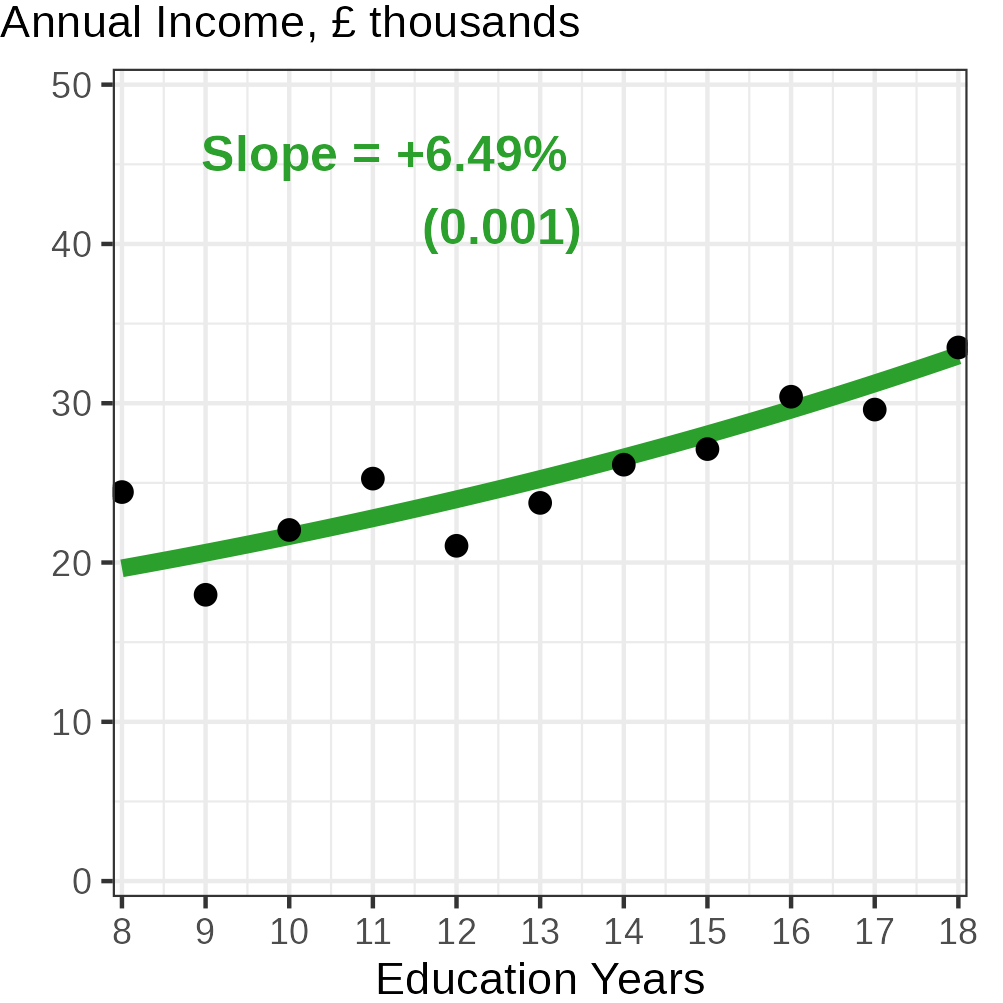
\includegraphics[width=\textwidth]{../text/sections/figures/edyears-earnings.png}
        \end{subfigure}
        \begin{subfigure}[b]{0.495\textwidth}
            \centering
            %\caption{Education Years $+$ Earnings.}
            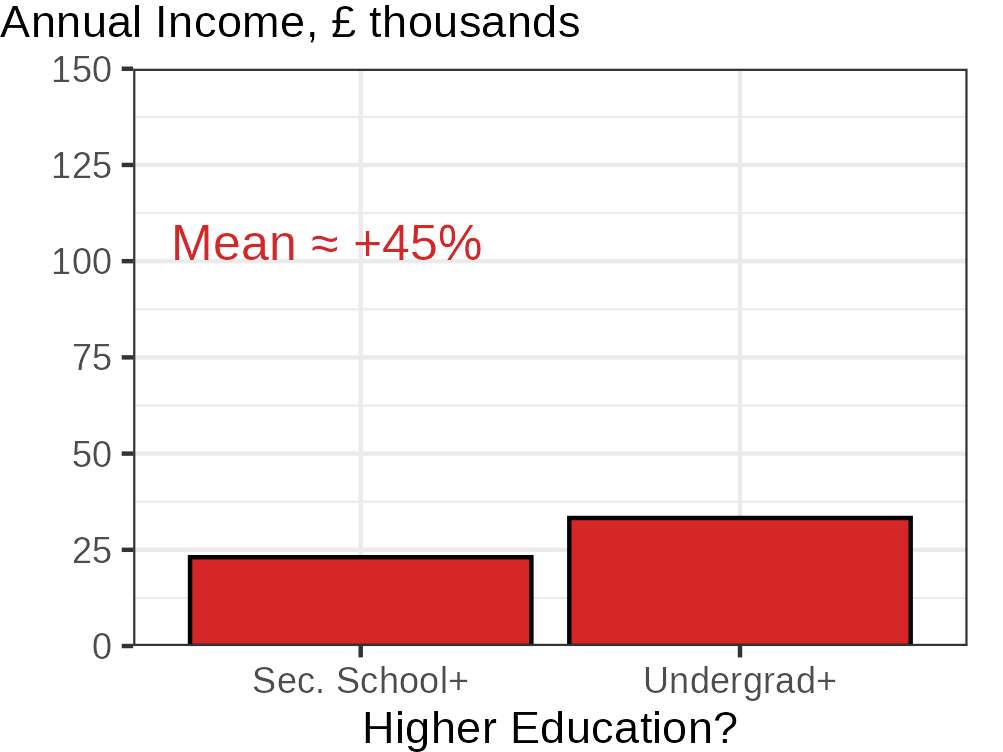
\includegraphics[width=\textwidth]{../text/sections/figures/college-earnings.png}
        \end{subfigure}
    \end{figure}
    \vspace{-0.25cm}
    $N = \input{../text/sections/tables/hrs-obs-count.txt}$ household heads with data on labour outcomes, age 50--65.\footnote[frame]{Limited to race $=$ white, for whom Ed PGI is defined.}
\end{frame}
%-------------------------------------------------------------------------------
\begin{frame}[noframenumbering]
    \frametitle{Data: Health \& Retirement Study}
    A representative panel of retirement-age Americans 1990--2021.
    \begin{figure}
        \centering
        \makebox[\textwidth][c]{
            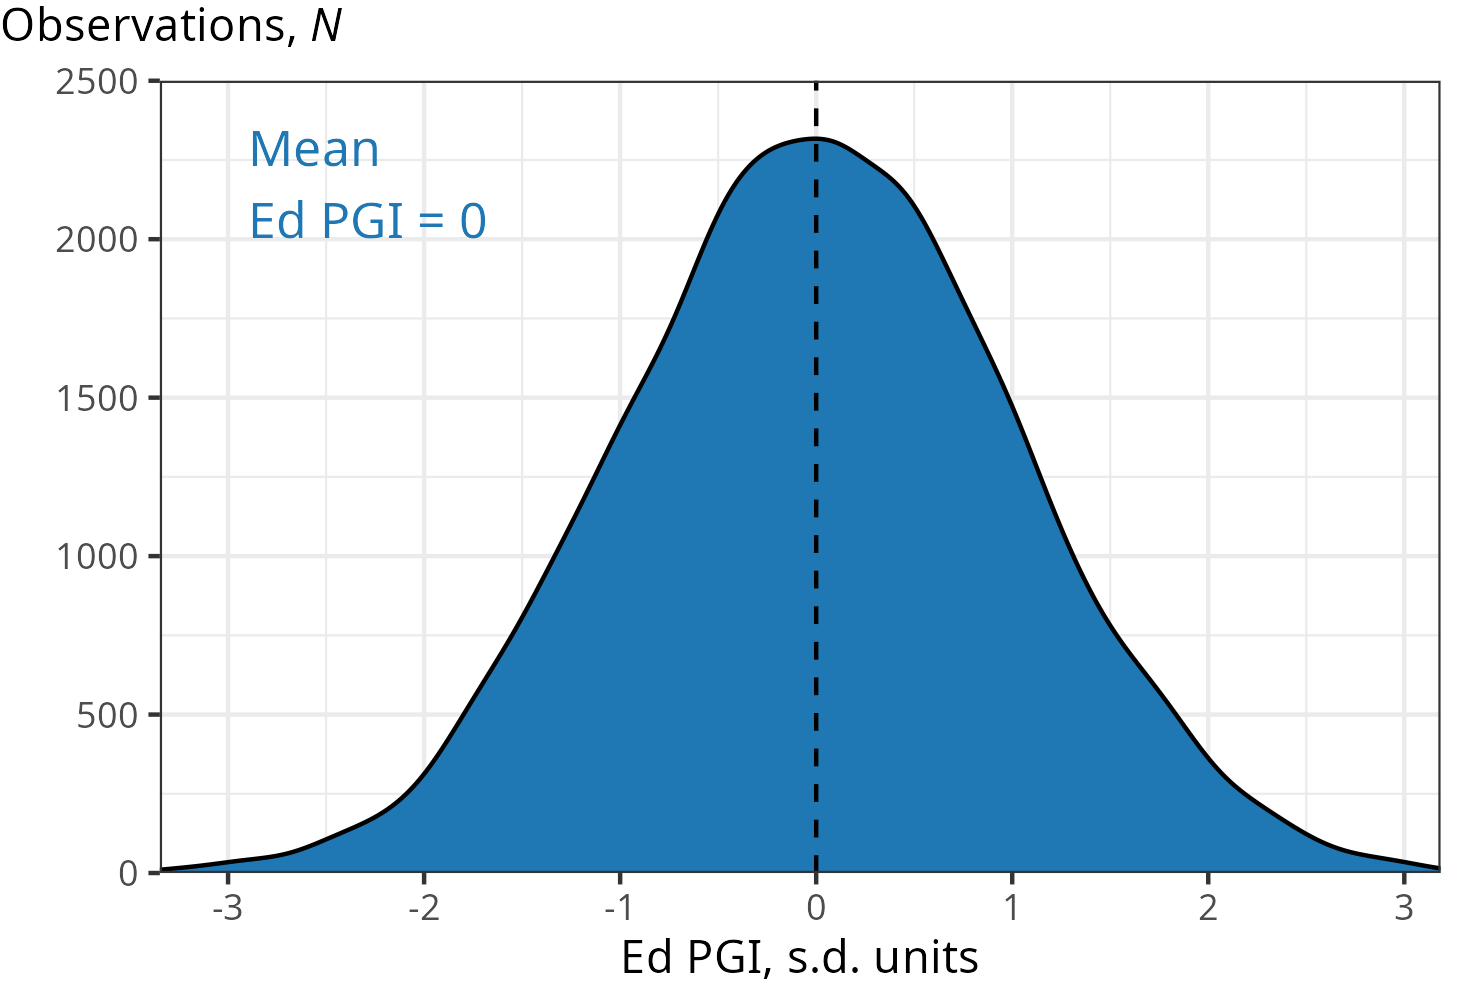
\includegraphics[width=0.75\textwidth]{
                ../text/sections/figures/genescore-hist-presentation.png}}
    \end{figure}
    \vspace{-0.25cm}
    $N = \input{../text/sections/tables/hrs-obs-count.txt}$ household heads with data on labour outcomes, age 50--65.\footnote[frame]{Limited to race $=$ white, for whom Ed PGI is defined.}
\end{frame}
%-------------------------------------------------------------------------------
\section{2. Genetic Effects}
\subsection{Mendelian Independent Assortment}
%-------------------------------------------------------------------------------
\begin{frame}
    \frametitle{Genetic Associations: Independent Assortment}
    \textbf{Question:} Is Ed PGI randomly assigned?
    \vspace{-0.25cm}
    \begin{figure}
        \centering
        \singlespacing
        \makebox[\textwidth][c]{
            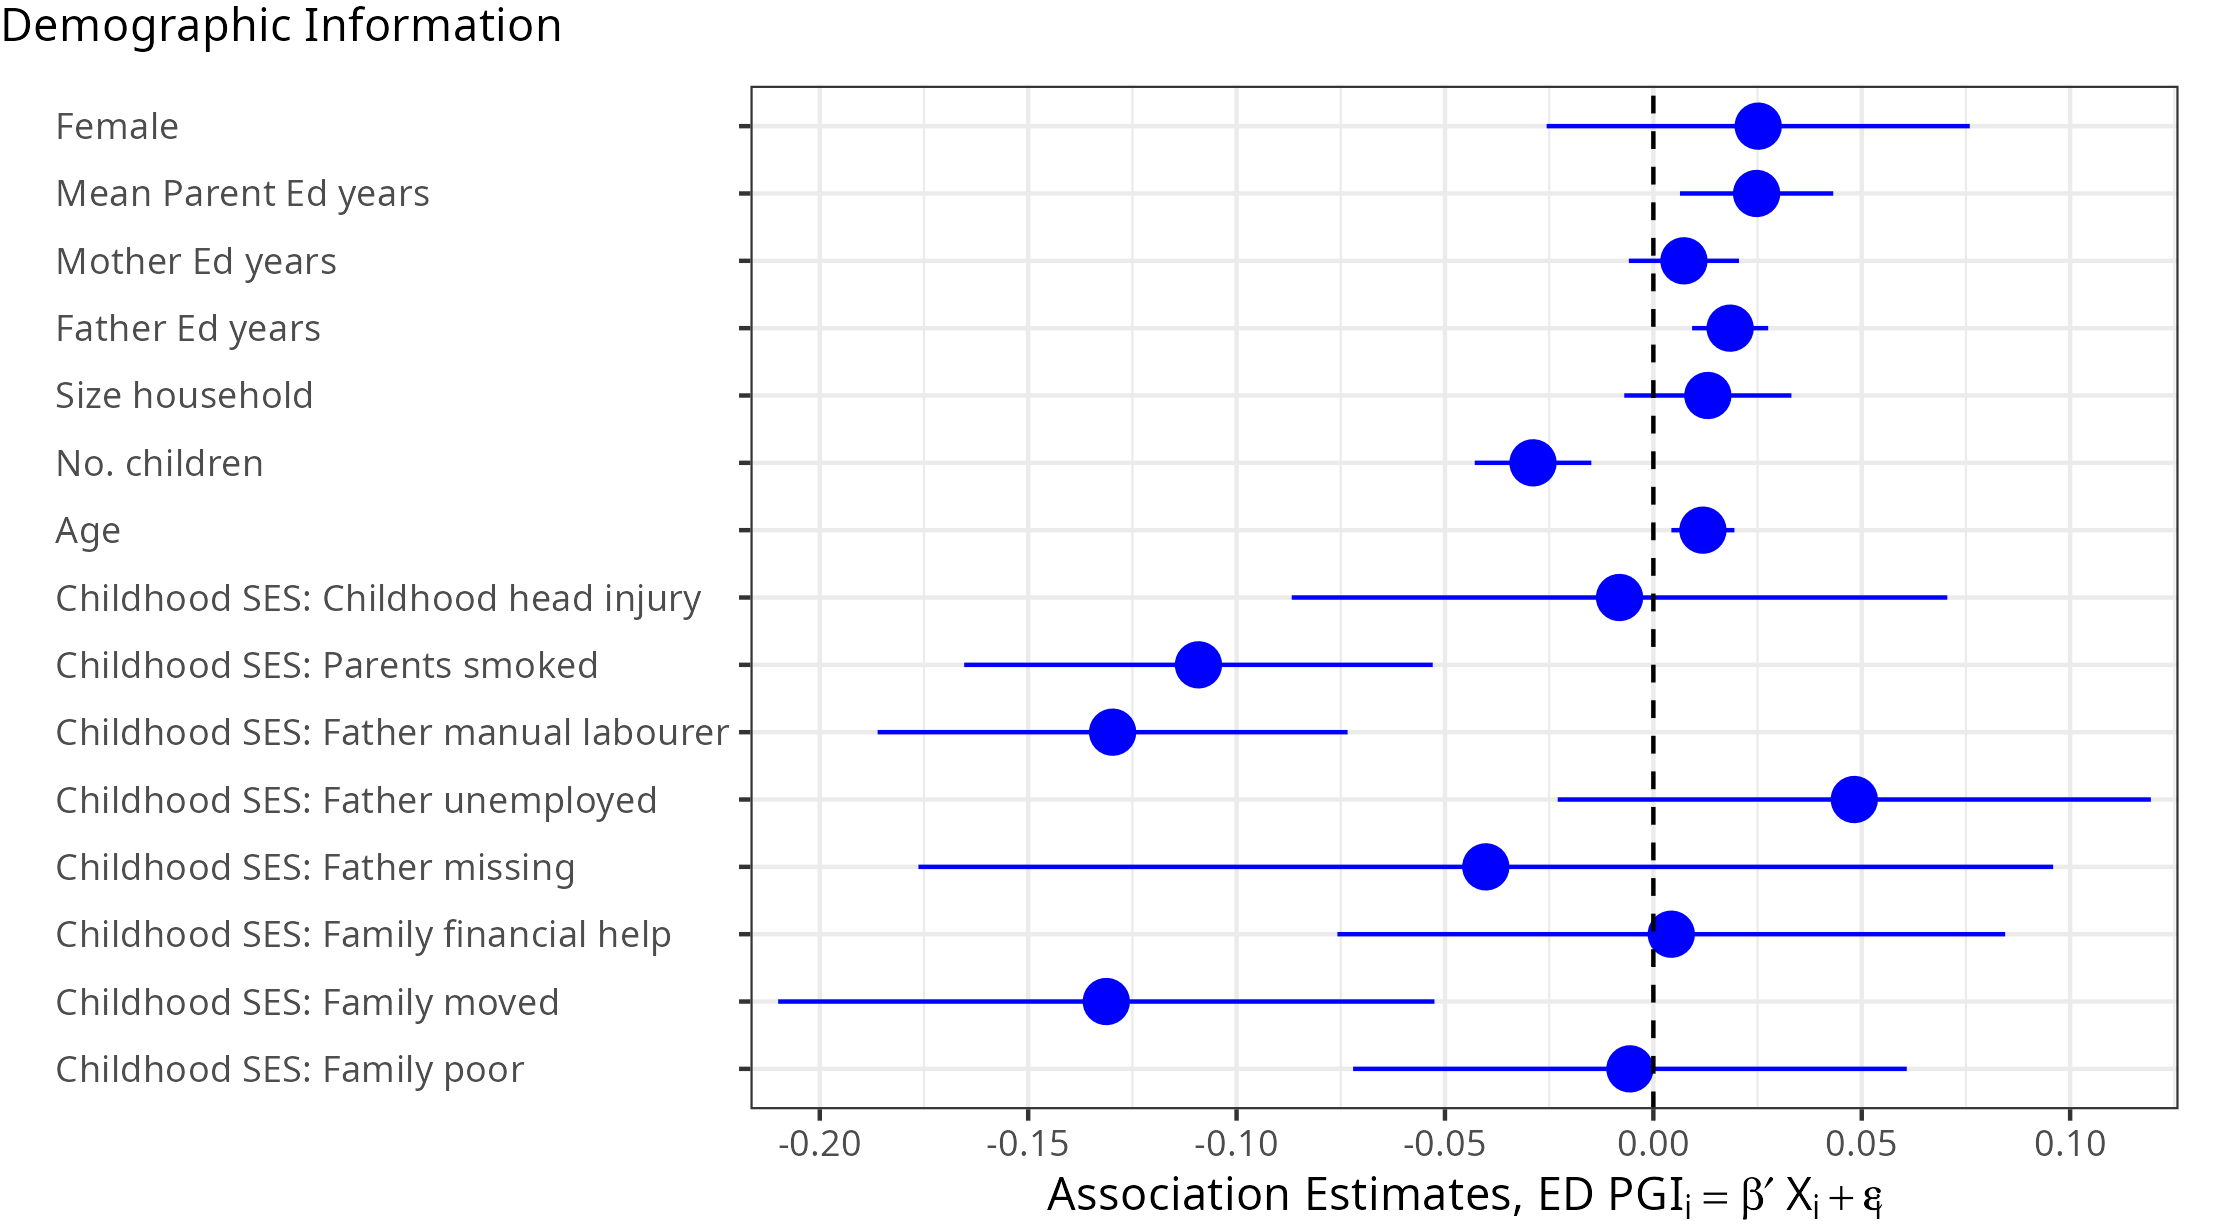
\includegraphics[width=\textwidth]{
                ../text/sections/figures/demographic-plot.png}}
    \end{figure}
\end{frame}
%-------------------------------------------------------------------------------
\begin{frame}[noframenumbering]
    \frametitle{Genetic Associations: Independent Assortment}
    \vspace{-0.25cm}
    \textbf{Question:} Is Ed PGI randomly assigned?

    \vspace{0.5cm}
    
    \begin{columns}
        \column{0.6\linewidth}
        \vspace{-0.7cm}

        \begin{figure}
            \raggedleft
            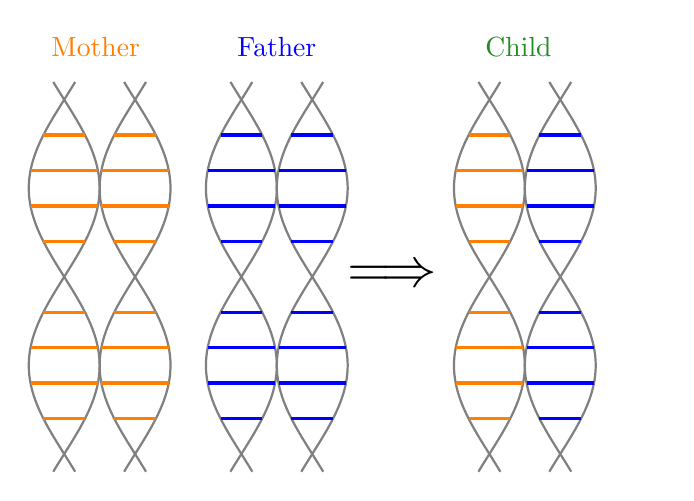
\begin{tikzpicture}
                % Draw the mother + father 
                \begin{scope}[scale=0.45, domain=-0.5:10.5, samples=110, rotate=90]
                    %% Father
                    \node[text width=1.0cm, color=blue] at (11.5, 0) {Father};
                    % Draw the phosphate backbone, for each chromosome.
                    \draw[gray, thick] plot (\x,{sin(\x*36) + 1});
                    \draw[gray, thick] plot (\x,{-sin(\x*36) + 1});
                    \draw[gray, thick] plot (\x,{sin(\x*36) - 1});
                    \draw[gray, thick] plot (\x,{-sin(\x*36) - 1});
                    % Draw the base pairs bonds
                    \foreach \x in {0, 1, ..., 10}{
                        \draw[very thick, blue] (\x, {-sin(\x*36) + 1}) -- (\x, {sin(\x*36) + 1});
                        \draw[very thick, blue] (\x, {-sin(\x*36) - 1}) -- (\x, {sin(\x*36) - 1});
                    }
                    %% Mother
                    \node[text width=1.0cm, color=orange] at (11.5, 0 + 5.25) {Mother};
                    % Draw the phosphate backbone for mother
                    \draw[gray, thick] plot (\x, {sin(\x*36) + 4});
                    \draw[gray, thick] plot (\x, {-sin(\x*36) + 4});
                    \draw[gray, thick] plot (\x, {sin(\x*36) + 6});
                    \draw[gray, thick] plot (\x, {-sin(\x*36) + 6});
                    % Draw the base pairs bonds
                    \foreach \x in {0, 1, ..., 10}{
                        \draw[very thick, orange] (\x, {-sin(\x*36) + 4}) -- (\x, {sin(\x*36) + 4});
                        \draw[very thick, orange] (\x, {-sin(\x*36) + 6}) -- (\x, {sin(\x*36) + 6});
                    }
                    %% Bridge to the child's genome
                    \node[text width=2cm, scale=2] at (5, -6) {$\implies$};
                    \node[text width=1.0cm, color=ForestGreen, scale=1] at (11.5, -7) {Child};
                    % Draw the phosphate backbone for child
                    \draw[gray, thick] plot (\x, {sin(\x*36) - 6});
                    \draw[gray, thick] plot (\x, {-sin(\x*36) - 6});
                    \draw[gray, thick] plot (\x, {sin(\x*36) - 8});
                    \draw[gray, thick] plot (\x, {-sin(\x*36) - 8});
                    % Draw base pairs bonds, one chromosome inherited from each
                    % Draw the base pairs bonds
                    \foreach \x in {0, 1, ..., 10}{
                        \draw[very thick, orange] (\x, {-sin(\x*36) - 6}) -- (\x, {sin(\x*36) - 6});
                        \draw[very thick, blue] (\x, {-sin(\x*36) - 8}) -- (\x, {sin(\x*36) - 8});
                    }
                \end{scope}
            \end{tikzpicture}
        \end{figure}
        \column{0.4\textwidth}
            \pause
            \textbf{Answer:}
            
            No, inherited from parents.
            \[ \Egiven{Z_i^\text{\textcolor{ForestGreen}{Child}}}{
                Z^\text{\textcolor{orange}{Mother}}_i,
                    Z^\text{\textcolor{blue}{Father}}_i
            } \]
            \[ = \frac 12 \left(
                Z^\text{\textcolor{orange}{Mother}}_i +
                    Z^\text{\textcolor{blue}{Father}}_i \right) \]
    \end{columns}
\end{frame}
%-------------------------------------------------------------------------------
\begin{frame}[noframenumbering]
    \frametitle{Genetic Associations: Independent Assortment}
    Difference in Ed PGI from parents' arises from random inheritance $+$ mixing, \textcolor{ForestGreen}{Mendelian Independent Assortment}.
    %\[ Z_i^\text{\textcolor{ForestGreen}{Child}}
    %    - \Egiven{Z_i^\text{\textcolor{ForestGreen}{Child}}}{
    %        Z^\text{\textcolor{orange}{Mother}}_i,
    %            Z^\text{\textcolor{blue}{Father}}_i
    %    } \;\; \longrightarrow \;\; \text{Independently assigned.} \]
    \begin{figure}
        \makebox[\textwidth][c]{
            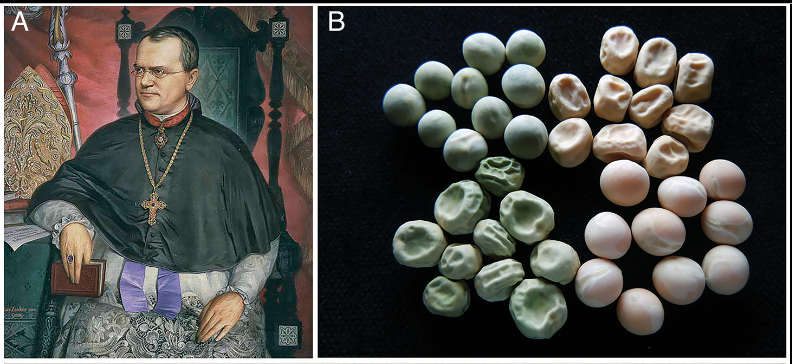
\includegraphics[width=0.75\textwidth]{
                presentation-files/headlines/mendels-pnas-1.png}}
    \end{figure}
    \vfill
    Abbot Mendel (1886) worked through principles of genetic inheritance 
    (Stenseth Andersson Hoekstra, 2022 PNAS).
\end{frame}
%-------------------------------------------------------------------------------
\begin{frame}[noframenumbering]
    \frametitle{Genetic Associations: Independent Assortment}
    Difference in Ed PGI from parents' arises from random inheritance $+$ mixing, \textcolor{ForestGreen}{Mendelian Independent Assortment}.
    \begin{figure}
        \makebox[\textwidth][c]{
            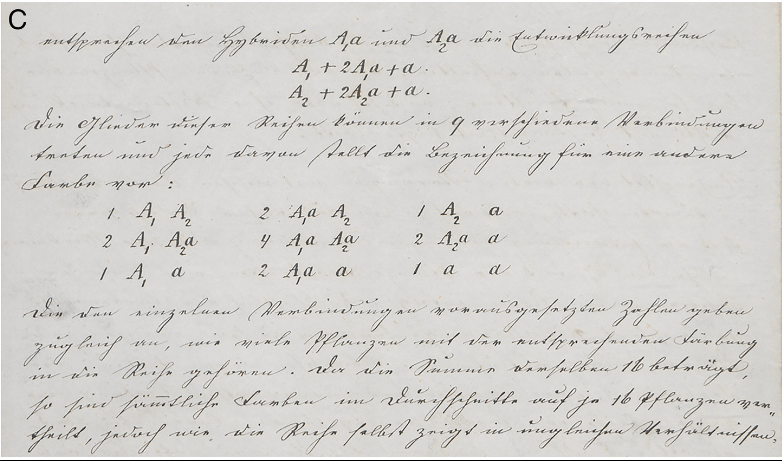
\includegraphics[width=0.65\textwidth]{
                presentation-files/headlines/mendels-pnas-2.png}}
    \end{figure}
    \vspace{0.25cm}

    Abbot Mendel (1886) worked through principles of genetic inheritance 
    (Stenseth Andersson Hoekstra, 2022 PNAS).
\end{frame}
%-------------------------------------------------------------------------------
\begin{frame}[noframenumbering]
    \frametitle{Genetic Associations: Independent Assortment}
    Difference in Ed PGI from parents' arises from random inheritance $+$ mixing, \textcolor{ForestGreen}{Mendelian Independent Assortment}.
    \begin{figure}
        \makebox[\textwidth][c]{
            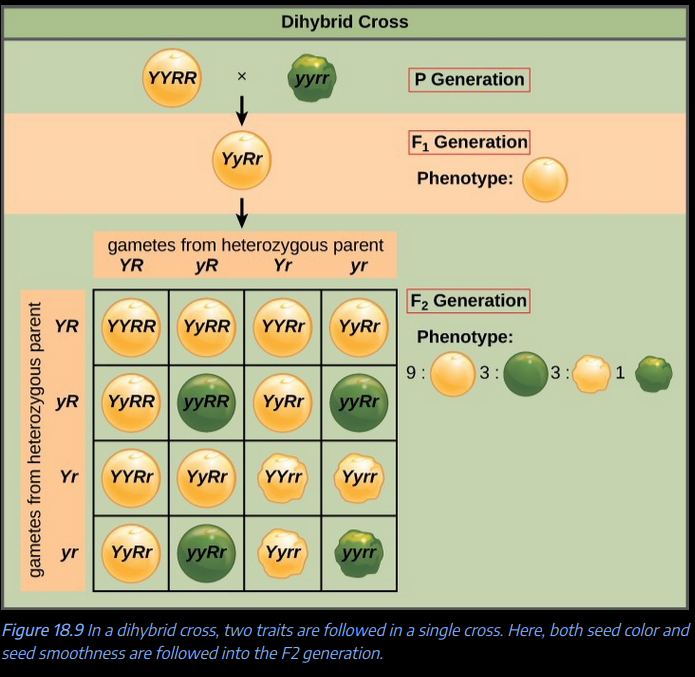
\includegraphics[width=0.5\textwidth]{
                presentation-files/headlines/mendels-peas.png}}
    \end{figure}
    \vfill
    Abbot Mendel (1886) worked through principles of genetic inheritance 
    (Stenseth Andersson Hoekstra, 2022 PNAS).
\end{frame}
%-------------------------------------------------------------------------------
\begin{frame}[noframenumbering]
    \frametitle{Genetic Associations: Independent Assortment}
    Difference in Ed PGI from parents' arises from random inheritance $+$ mixing, \textcolor{ForestGreen}{Mendelian Independent Assortment}.
    \begin{columns}
        \column{0.375\linewidth}
        \vspace{-0.75cm}

        \begin{figure}
            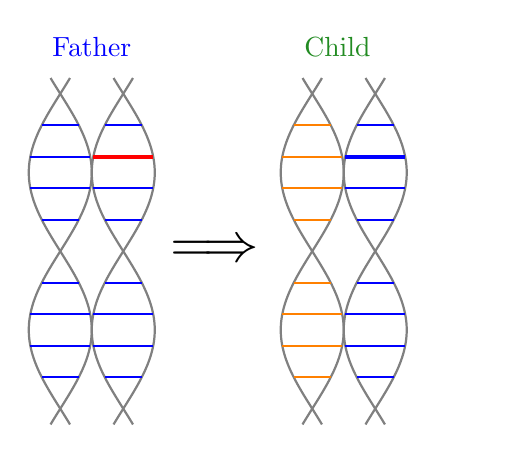
\begin{tikzpicture}
                % Draw the father's two copies of the genes.
                \begin{scope}[scale=0.4, domain=-0.5:10.5, samples=110, rotate=90]
                    %% Father
                    \node[color=blue] at (11.5, -1) {Father};
                    % Draw the phosphate backbone for father's first chromosome.
                    \draw[gray, thick] plot (\x,{sin(\x*36)});
                    \draw[gray, thick] plot (\x,{-sin(\x*36)});
                    % Draw the phosphate backbone for father's second chromosome.
                    \draw[gray, thick] plot (\x, {sin(\x*36) - 2});
                    \draw[gray, thick] plot (\x, {-sin(\x*36) - 2});
                    % Draw the base pairs bonds (missing mutation at j = 8)
                    \foreach \x in {0, 1, ..., 7, 9, 10}{
                        \draw[blue, thick] (\x, {-sin(\x*36)}) -- (\x, {sin(\x*36)});
                        \draw[blue, thick] (\x, {-sin(\x*36) - 2}) -- (\x, {sin(\x*36) - 2});
                    }
                    % Draw the father's mutation at j = 8, only on second chromosome
                    \foreach \x in {8}{
                        \draw[blue, thick] (\x, {-sin(\x*36)}) -- (\x, {sin(\x*36)});
                        \draw[red, ultra thick] (\x, {-sin(\x*36) - 2}) -- (\x, {sin(\x*36) - 2});
                    }
                    %% Bridge to the child's genome
                    \node[text width=2cm, scale=2] at (5, -8) {$\implies$};
                    \node[text width=1.0cm, color=ForestGreen, scale=1] at (11.5, -9) {Child};
                    % Draw the phosphate backbone for child's first chromosome.
                    \draw[gray, thick] plot (\x, {sin(\x*36) - 8});
                    \draw[gray, thick] plot (\x, {-sin(\x*36) - 8});
                    % Draw the phosphate backbone for child's second chromosome.
                    \draw[gray, thick] plot (\x, {sin(\x*36) - 10});
                    \draw[gray, thick] plot (\x, {-sin(\x*36) - 10});
                    % Draw the base pairs bonds (missing mutation at j = 8)
                    \foreach \x in {0, 1, ..., 7, 8, 9, 10}{
                        \draw[orange, thick] (\x, {-sin(\x*36) - 8}) -- (\x, {sin(\x*36) - 8});
                        \draw[blue, thick] (\x, {-sin(\x*36) - 10}) -- (\x, {sin(\x*36) - 10});
                    }
                    % Draw the optional mutation at j = 8.
                    \foreach \x in {8}{
                        \draw[blue, ultra thick] (\x, {-sin(\x*36) - 10}) -- (\x, {sin(\x*36) - 10});
                        %\draw[white] (\x, {-sin(\x*36) - 10}) -- (\x, {sin(\x*36) - 10});
                    }
                \end{scope}
            \end{tikzpicture}
        \end{figure}
        \column{0.525\textwidth}
            \[ \Pr \big(
                \text{\textcolor{ForestGreen}{Child} inherits} \; \big| \;
                \text{\textcolor{blue}{Father} one copy} \big)
                = \frac 12 \]
            I.e., inheritance prop. score identified.

            \vspace{0.5cm}
            \begin{colormixin}{15!bg}
            Propagate this reasoning across all \textcolor{red}{1,271 single-letter changes} in the Ed PGI, and both parents:
            \end{colormixin}
    \end{columns}
    \begin{colormixin}{15!bg}
    \[ Z_i^\text{\textcolor{ForestGreen}{Child}}
        - \Egiven{Z_i^\text{\textcolor{ForestGreen}{Child}}}{
            Z^\text{\textcolor{blue}{Father}}_i,
                Z^\text{\textcolor{orange}{Mother}}_i
        } \;\; \longrightarrow \;\; \text{Independently assigned.} \]
    \end{colormixin}
\end{frame}
%-------------------------------------------------------------------------------
\begin{frame}[noframenumbering]
    \frametitle{Genetic Associations: Independent Assortment}
    \vspace{-0.125cm}

    Difference in Ed PGI from parents' arises from random inheritance $+$ mixing, \textcolor{ForestGreen}{Mendelian Independent Assortment}.
    \begin{columns}
        \column{0.375\linewidth}
        \vspace{-0.75cm}

        \begin{figure}
            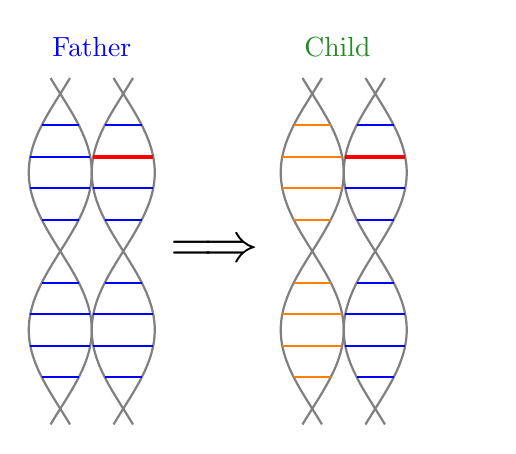
\begin{tikzpicture}
                % Draw the father's two copies of the genes.
                \begin{scope}[scale=0.4, domain=-0.5:10.5, samples=110, rotate=90]
                    %% Father
                    \node[color=blue] at (11.5, -1) {Father};
                    % Draw the phosphate backbone for father's first chromosome.
                    \draw[gray, thick] plot (\x,{sin(\x*36)});
                    \draw[gray, thick] plot (\x,{-sin(\x*36)});
                    % Draw the phosphate backbone for father's second chromosome.
                    \draw[gray, thick] plot (\x, {sin(\x*36) - 2});
                    \draw[gray, thick] plot (\x, {-sin(\x*36) - 2});
                    % Draw the base pairs bonds (missing mutation at j = 8)
                    \foreach \x in {0, 1, ..., 7, 9, 10}{
                        \draw[blue, thick] (\x, {-sin(\x*36)}) -- (\x, {sin(\x*36)});
                        \draw[blue, thick] (\x, {-sin(\x*36) - 2}) -- (\x, {sin(\x*36) - 2});
                    }
                    % Draw the father's mutation at j = 8, only on second chromosome
                    \foreach \x in {8}{
                        \draw[blue, thick] (\x, {-sin(\x*36)}) -- (\x, {sin(\x*36)});
                        \draw[red, ultra thick] (\x, {-sin(\x*36) - 2}) -- (\x, {sin(\x*36) - 2});
                    }
                    %% Bridge to the child's genome
                    \node[text width=2cm, scale=2] at (5, -8) {$\implies$};
                    \node[text width=1.0cm, color=ForestGreen, scale=1] at (11.5, -9) {Child};
                    % Draw the phosphate backbone for child's first chromosome.
                    \draw[gray, thick] plot (\x, {sin(\x*36) - 8});
                    \draw[gray, thick] plot (\x, {-sin(\x*36) - 8});
                    % Draw the phosphate backbone for child's second chromosome.
                    \draw[gray, thick] plot (\x, {sin(\x*36) - 10});
                    \draw[gray, thick] plot (\x, {-sin(\x*36) - 10});
                    % Draw the base pairs bonds (missing mutation at j = 8)
                    \foreach \x in {0, 1, ..., 7, 8, 9, 10}{
                        \draw[orange, thick] (\x, {-sin(\x*36) - 8}) -- (\x, {sin(\x*36) - 8});
                        \draw[blue, thick] (\x, {-sin(\x*36) - 10}) -- (\x, {sin(\x*36) - 10});
                    }
                    % Draw the optional mutation at j = 8
                    \foreach \x in {8}{
                        \draw[red, ultra thick] (\x, {-sin(\x*36) - 10}) -- (\x, {sin(\x*36) - 10});
                        %\draw[white] (\x, {-sin(\x*36) - 10}) -- (\x, {sin(\x*36) - 10});
                    }
                \end{scope}
            \end{tikzpicture}
        \end{figure}
        \column{0.525\textwidth}
            \[ \Pr \big(
                \text{\textcolor{ForestGreen}{Child} inherits} \; \big| \;
                \text{\textcolor{blue}{Father} one copy} \big)
                = \frac 12 \]
            I.e., inheritance prop. score identified.

            \vspace{0.5cm}
            \pause
            Propagate this reasoning across all \textcolor{red}{1,271 single-letter changes} in the Ed PGI, and both parents:
    \end{columns}
    \[ Z_i^\text{\textcolor{ForestGreen}{Child}}
        - \Egiven{Z_i^\text{\textcolor{ForestGreen}{Child}}}{
            Z^\text{\textcolor{blue}{Father}}_i,
                Z^\text{\textcolor{orange}{Mother}}_i
        } \;\; \longrightarrow \;\; \text{Independently assigned.} \]
\end{frame}
%-------------------------------------------------------------------------------
\begin{frame}[noframenumbering]
    \frametitle{Genetic Associations: Independent Assortment}
    \vspace{-0.125cm}

    Difference in Ed PGI from parents' arises from random inheritance $+$ mixing, \textcolor{ForestGreen}{Mendelian Independent Assortment}.
    \vspace{0.25cm}
    \begin{figure}
        \centering
        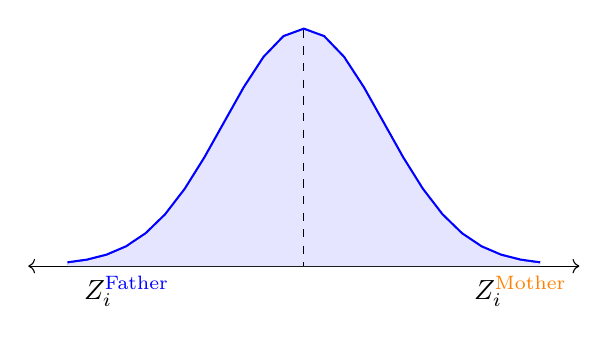
\begin{tikzpicture}
            % define normal distribution function ``normal''
            \def\normalheight{3.0}
            \def\normaldist{\x,{3.0 * exp((-(\x)^2) / 2)}}
            % Draw the x-axis
            \draw[<->] (-3.5,0) -- (3.5,0);
            % Draw and label normal distribution function
            \draw[ultra thick,color=blue,domain=-3:3] plot (\normaldist);
            \fill [fill=blue!10] (-3,0) -- plot[domain=-3:3] (\normaldist) -- (3,0) -- cycle;
            % Add dashed line dropping down from normal, at mean = 0
            \draw[dashed] (0,{\normalheight}) -- (0,0);
            % Label Mother and father's values, at extreme end of the distribution.
            \node[below] at (2.75,0) {$Z^\text{\textcolor{orange}{Mother}}_i$};
            \node[below] at (-2.25,0) {$Z^\text{\textcolor{blue}{Father}}_i$};
        \end{tikzpicture}
    \end{figure}
    \vspace{0.25cm}

    Propagate this reasoning across all \textcolor{red}{1,271 single-letter changes} in the Ed PGI, and both parents:
    \[ Z_i^\text{\textcolor{ForestGreen}{Child}}
        - \Egiven{Z_i^\text{\textcolor{ForestGreen}{Child}}}{
            Z^\text{\textcolor{blue}{Father}}_i,
                Z^\text{\textcolor{orange}{Mother}}_i
        } \;\; \longrightarrow \;\; \text{Independently assigned.} \]
\end{frame}
%-------------------------------------------------------------------------------
\begin{frame}[noframenumbering]
    \frametitle{Genetic Associations: Independent Assortment}
    \vspace{-0.125cm}

    Difference in Ed PGI from parents' arises from random inheritance $+$ mixing, \textcolor{ForestGreen}{Mendelian Independent Assortment}.
    \vspace{0.25cm}
    \begin{figure}
        \centering
        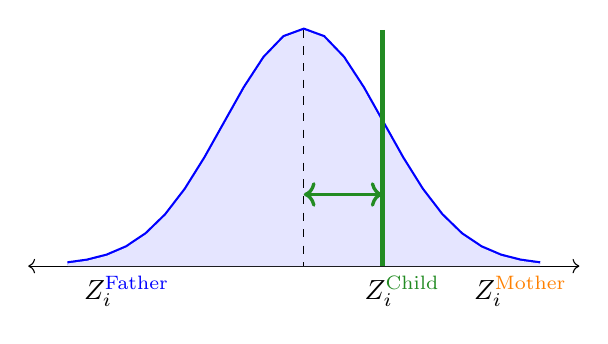
\begin{tikzpicture}
            % define normal distribution function ``normal''
            \def\normalheight{3.0}
            \def\normaldist{\x,{3.0 * exp((-(\x)^2) / 2)}}
            % Draw the x-axis
            \draw[<->] (-3.5,0) -- (3.5,0);
            % Draw and label normal distribution function
            \draw[ultra thick,color=blue,domain=-3:3] plot (\normaldist);
            \fill [fill=blue!10] (-3,0) -- plot[domain=-3:3] (\normaldist) -- (3,0) -- cycle;
            % Add dashed line dropping down from normal, at mean = 0
            \draw[dashed] (0,{\normalheight}) -- (0,0);
            % Label Mother and father's values, at extreme end of the distribution.
            \node[below] at (2.75,0) {$Z^\text{\textcolor{orange}{Mother}}_i$};
            \node[below] at (-2.25,0) {$Z^\text{\textcolor{blue}{Father}}_i$};
            % Label the Child's resulting value
            \def\childvalue{1}
            \def\childnormalheight{{(3.0 / 2) * exp((-(1)^2) / 2)}}
            \draw[ultra thick,color=ForestGreen] ({\childvalue},{\normalheight}) -- ({\childvalue},0);
            \node[below] at ({\childvalue + 0.25},0) {$Z_i^\text{\textcolor{ForestGreen}{Child}}$};
            \draw[<->,very thick,color=ForestGreen] (0, {\childnormalheight}) -- (\childvalue, {\childnormalheight});
        \end{tikzpicture}
    \end{figure}
    \vspace{0.25cm}

    Propagate this reasoning across all \textcolor{red}{1,271 single-letter changes} in the Ed PGI, and both parents:
    \[ Z_i^\text{\textcolor{ForestGreen}{Child}}
        - \Egiven{Z_i^\text{\textcolor{ForestGreen}{Child}}}{
            Z^\text{\textcolor{blue}{Father}}_i,
                Z^\text{\textcolor{orange}{Mother}}_i
        } \;\; \longrightarrow \;\; \text{Independently assigned.} \]
\end{frame}

%-------------------------------------------------------------------------------
\begin{frame}[noframenumbering]
    \frametitle{Genetic Associations: Independent Assortment}
    \vspace{-0.125cm}

    Difference in Ed PGI from parents' arises from random inheritance $+$ mixing, \textcolor{ForestGreen}{Mendelian Independent Assortment}.
    \vspace{0.25cm}
    \begin{figure}
        \centering
        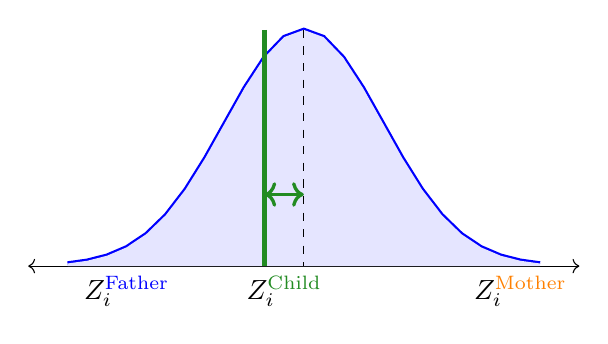
\begin{tikzpicture}
            % define normal distribution function ``normal''
            \def\normalheight{3.0}
            \def\normaldist{\x,{3.0 * exp((-(\x)^2) / 2)}}
            % Draw the x-axis
            \draw[<->] (-3.5,0) -- (3.5,0);
            % Draw and label normal distribution function
            \draw[ultra thick,color=blue,domain=-3:3] plot (\normaldist);
            \fill [fill=blue!10] (-3,0) -- plot[domain=-3:3] (\normaldist) -- (3,0) -- cycle;
            % Add dashed line dropping down from normal, at mean = 0
            \draw[dashed] (0,{\normalheight}) -- (0,0);
            % Label Mother and father's values, at extreme end of the distribution.
            \node[below] at (2.75,0) {$Z^\text{\textcolor{orange}{Mother}}_i$};
            \node[below] at (-2.25,0) {$Z^\text{\textcolor{blue}{Father}}_i$};
            % Label the Child's resulting value
            \def\childvalue{-0.5}
            \def\childnormalheight{{(3.0 / 2) * exp((-(1)^2) / 2)}}
            \draw[ultra thick,color=ForestGreen] ({\childvalue},{\normalheight}) -- ({\childvalue},0);
            \node[below] at ({\childvalue + 0.25},0) {$Z_i^\text{\textcolor{ForestGreen}{Child}}$};
            \draw[<->,very thick,color=ForestGreen] (0, {\childnormalheight}) -- (\childvalue, {\childnormalheight});
        \end{tikzpicture}
    \end{figure}
    \vspace{0.25cm}

    Propagate this reasoning across all \textcolor{red}{1,271 single-letter changes} in the Ed PGI, and both parents:
    \[ Z_i^\text{\textcolor{ForestGreen}{Child}}
        - \Egiven{Z_i^\text{\textcolor{ForestGreen}{Child}}}{
            Z^\text{\textcolor{blue}{Father}}_i,
                Z^\text{\textcolor{orange}{Mother}}_i
        } \;\; \longrightarrow \;\; \text{Independently assigned.} \]
\end{frame}
%-------------------------------------------------------------------------------
\begin{frame}[noframenumbering]
    \frametitle{Genetic Associations: Independent Assortment}
    \vspace{-0.125cm}

    Difference in Ed PGI from parents' arises from random inheritance $+$ mixing, \textcolor{ForestGreen}{Mendelian Independent Assortment}.
    \vspace{0.5cm}

    \begin{columns}
        \column{0.375\linewidth}
        \vspace{-0.75cm}
        \centering
        \begin{figure}
            \resizebox{1.1\linewidth}{0.75\linewidth}{
            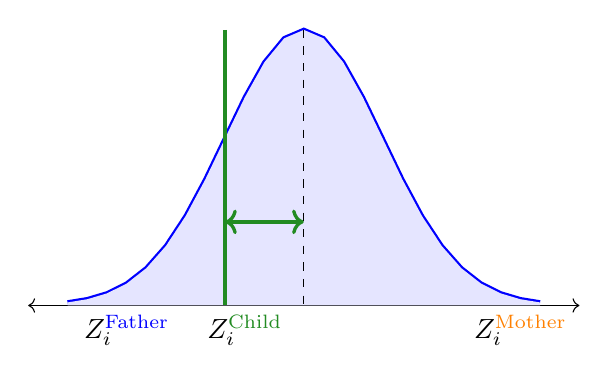
\begin{tikzpicture}
                % define normal distribution function ``normal''
                \def\normalheight{3.5}
                \def\normaldist{\x,{3.5 * exp((-(\x)^2) / 2)}}
                % Draw the x-axis
                \draw[<->] (-3.5,0) -- (3.5,0);
                % Draw and label normal distribution function
                \draw[ultra thick,color=blue,domain=-3:3] plot (\normaldist);
                \fill [fill=blue!10] (-3,0) -- plot[domain=-3:3] (\normaldist) -- (3,0) -- cycle;
                % Add dashed line dropping down from normal, at mean = 0
                \draw[dashed] (0,{\normalheight}) -- (0,0);
                % Label Mother and father's values, at extreme end of the distribution.
                \node[below] at (2.75,0) {$Z^\text{\textcolor{orange}{Mother}}_i$};
                \node[below] at (-2.25,0) {$Z^\text{\textcolor{blue}{Father}}_i$};
                % Label the Child's resulting value
                \def\childvalue{-1}
                \def\childnormalheight{{(3.5 / 2) * exp((-(1)^2) / 2)}}
                \draw[ultra thick,color=ForestGreen] ({\childvalue},{\normalheight}) -- ({\childvalue},0);
                \node[below] at ({\childvalue + 0.25},0) {$Z_i^\text{\textcolor{ForestGreen}{Child}}$};
                \draw[<->,very thick,color=ForestGreen] (0, {\childnormalheight}) -- (\childvalue, {\childnormalheight});
            \end{tikzpicture}}
        \end{figure}
        \column{0.525\textwidth}
            $\implies$ Use the difference from parents as \textcolor{blue}{plausibly random genetic variation}.
            \[ Z_i^\text{\textcolor{ForestGreen}{Child}}
            - \Egiven{Z_i^\text{\textcolor{ForestGreen}{Child}}}{
                Z^\text{\textcolor{orange}{Mother}}_i,
                    Z^\text{\textcolor{blue}{Father}}_i} \]
            \pause
            
            \textbf{Remark on Identification:} \\
            Equivalent to instrumenting \textcolor{ForestGreen}{Child}'s Ed PGI
            using deviation from parents \\
            (e.g., formula instrument).
    \end{columns}
    \pause
    \vspace{0.5cm}

    \textbf{LWIPS Note:} UK Biobank has data on a few thousand people linked to parent/siblings.
    Look forward to results using these data $+$ design in 2025.
    % Put a figure which shows the further apart parents are, then more room to get a random choice.
    % Normal dist between Min{Z father, Z Mother} and Max{Z father, Z Mother}, with mean at the half-way point.
    % And perhaps fat tails above/below maxi/min, respectively.
\end{frame}
%-------------------------------------------------------------------------------
\begin{frame}
    \frametitle{Genetic Associations: Outcomes}
    \textbf{Question:} Is Ed PGI related to labour market outcomes?
    
    \vspace{-0.5cm}
    \begin{figure}
        \centering
        \singlespacing
        
\begin{tikzpicture}
            \node[state,blue] (instrument) at (0,0) {$Z$};
            \node[state,ForestGreen] (outcome) [right=1.5cm of instrument] {$D$};
            \path[->] (instrument) edge (outcome);
            % Label the nodes with econ examples
            \node[color=blue] [left=0.1cm of instrument] {Ed PGI};
            \node[text width=0.1cm, color=ForestGreen] [right=-0.01cm of outcome] {Education};
        \end{tikzpicture}
    \end{figure}
    \vspace{-0.25cm}
    \begin{figure}
        \centering
        \caption{Bin Scatter Between \textcolor{blue}{Ed PGI}
            $+$ \textcolor{ForestGreen}{Education Years}.}
        \makebox[\textwidth][c]{
            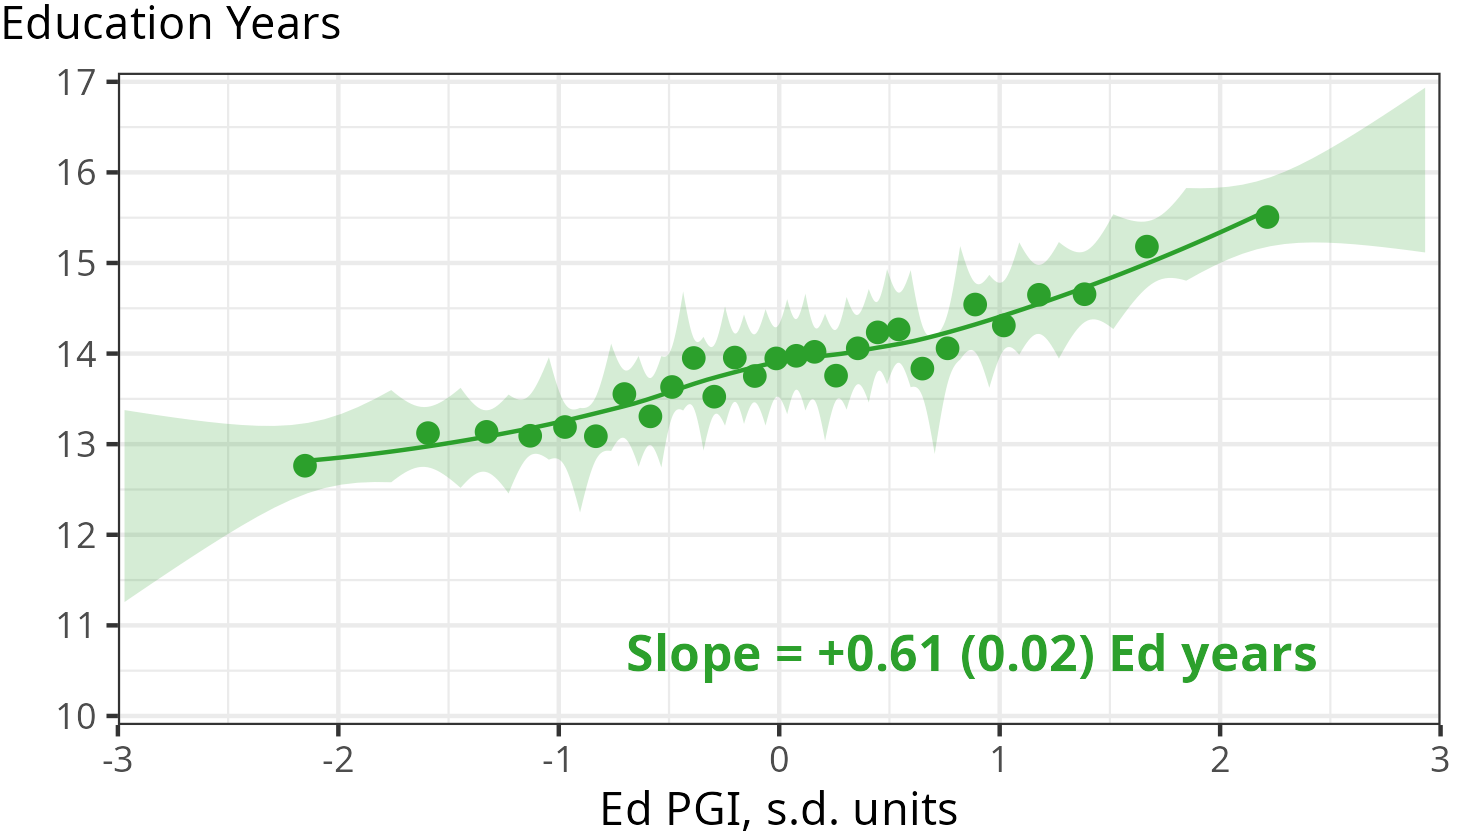
\includegraphics[width=0.8\textwidth]{
                ../text/sections/figures/genescore-edyears-wider.png}}
    \end{figure}
\end{frame}
%-------------------------------------------------------------------------------
\begin{frame}[noframenumbering]
    \frametitle{Genetic Associations: Outcomes}
    \textbf{Question:} Is Ed PGI related to labour market outcomes?

    \vspace{-0.5cm}
    \begin{figure}
        \centering
        \singlespacing
        
\begin{tikzpicture}
            \node[state,blue] (instrument) at (0,0) {$Z$};
            \node[state,red] (outcome) [right=1.5cm of instrument] {$Y$};
            \path[->] (instrument) edge (outcome);
            % Label the nodes with econ examples
            \node[color=blue] [left=0.1cm of instrument] {Ed PGI};
            \node[text width=0.1cm, color=red] [right=-0.01cm of outcome] {Earnings};
        \end{tikzpicture}
    \end{figure}
    \vspace{-0.25cm}
    \begin{figure}
        \centering
        \caption{Bin Scatter Between \textcolor{blue}{Ed PGI}
            $+$ \textcolor{red}{Annual Earnings.}}
        \makebox[\textwidth][c]{
            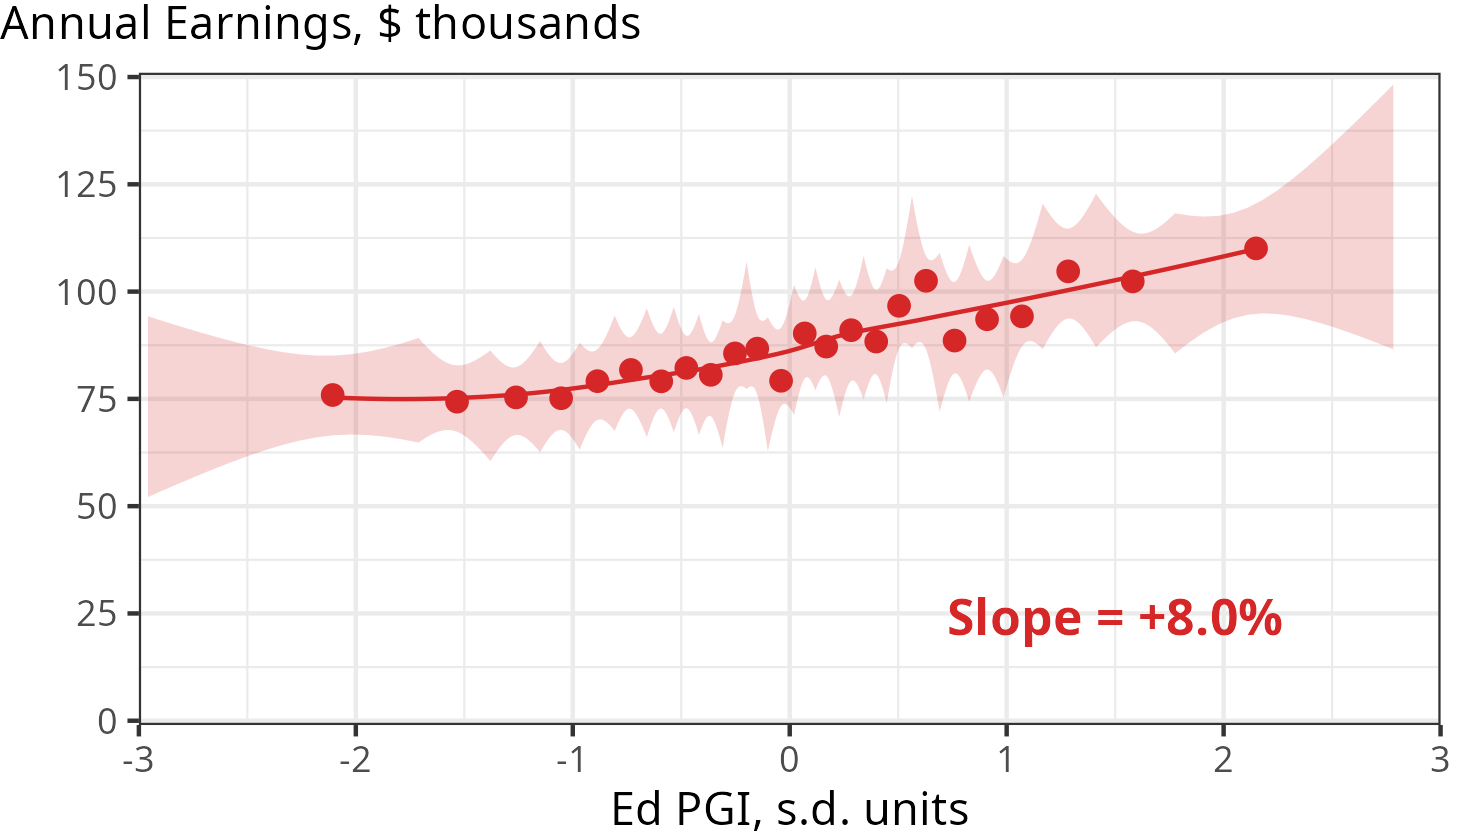
\includegraphics[width=0.8\textwidth]{
                ../text/sections/figures/genescore-earnings-wider}}
    \end{figure}
\end{frame}
%-------------------------------------------------------------------------------
\section{3. Direct and Indirect Effects}
%-------------------------------------------------------------------------------
\begin{frame}
    \frametitle{Direct and Indirect Effects}
    Ed PGI is correlated with \textbf{education and income}, so what?
    \pause

    $\to$ Ed PGI computed from training data on \textbf{only genes $+$ education}.
    \vspace{-0.35cm}
    \begin{figure}
        \centering
        \singlespacing
        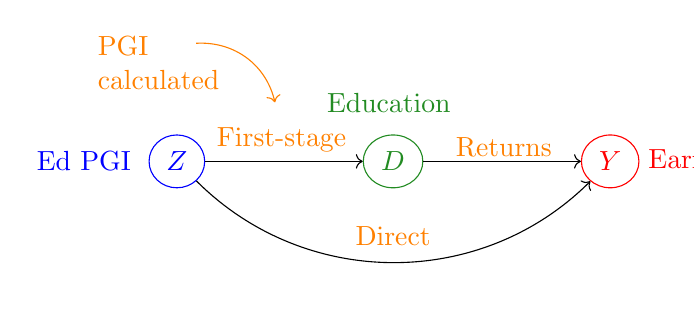
\begin{tikzpicture}
            \node[state,ForestGreen] (treatment) at (0,0) {$D$};
            \node[state,blue] (instrument) [left=2cm of treatment] {$Z$};
            \path[->] (instrument) edge (treatment);
            \node[color=blue] [left=0.1cm of instrument] {Ed PGI};
            \node[text width=1.675cm, color=ForestGreen] [above=0.15cm of treatment] (education) {Education};
            \node[text height=0.5cm, color=orange] [above left=-0.25cm and 0.2cm of treatment] {First-stage};
            % Label where Ed PGI is computed
            \path[->, color=orange] (-2.5, 1.5) edge[bend left=40] (-1.5, 0.75);
            \node[text width=2cm, color=orange] at (-2.75, 1.25) {PGI\\calculated};
            % Add in direct effects.
            \pause
            \node[state,red] (outcome) [right=2cm of treatment] {$Y$};
            \node[text width=0.1cm, color=red] [right=-0.01cm of outcome] {Earnings};
            \path[->] (instrument) edge[bend right=45] (outcome);
            \node[text height=0.25cm, color=orange] [below=0.35cm of treatment] {Direct};
            % Add on returns to education.
            \pause
            \path[->] (treatment) edge (outcome);
            \node[text height=0.5cm, color=orange] [above right=-0.3 and 0.4cm of treatment] {Returns};
        \end{tikzpicture}
    \end{figure}

    \vspace{-0.25cm}
    \pause
    $\implies$ Association with earnings is non-trivial, can operate two channels:
    %\vspace{-0.5cm}
    \begin{table}
        \centering
        \begin{tabular}{p{0.45\textwidth} | p{0.45\textwidth}}
            \textcolor{orange}{Direct Genetic Channel} &
                \textcolor{orange}{Returns to Education} \\ \hline
            \begin{itemize}
                \item Creativity $+$ Soft skills
                \item Correlation with first-stage
                \item Signalling(?)
            \end{itemize} &
            \begin{itemize}
                \item Classroom learning
                \item Hard skills
                \item Occupational qualifications
            \end{itemize}
        \end{tabular}
    \end{table}
\end{frame}
%-------------------------------------------------------------------------------
\subsection{Ed PGI's Effects Through Education}
%-------------------------------------------------------------------------------
\begin{frame}
    \frametitle{Direct and Indirect Effects}
    Mediation methods are a general-purpose tool to decompose total treatment effect: \textcolor{blue}{Direct} $+$ \textcolor{ForestGreen}{Indirect} effects.
    \vspace{-0.5cm}
    \begin{figure}
        \centering
        \singlespacing
        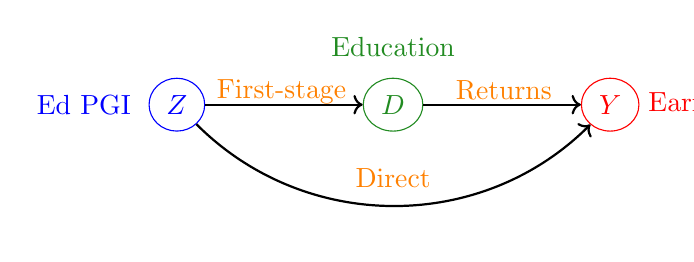
\begin{tikzpicture}
            \node[state,ForestGreen] (treatment) at (0,0) {$D$};
            \node[state,blue] (instrument) [left=2cm of treatment] {$Z$};
            \node[state,red] (outcome) [right=2cm of treatment] {$Y$};
            % Label Z, D, Y
            \node[color=ForestGreen] [above=0.15cm of treatment] (education) {Education};
            \node[color=blue] [left=0.1cm of instrument] {Ed PGI};
            \node[text width=0.1cm, color=red] [right=-0.01cm of outcome] {Earnings};
            % Draw the causal arrows
            \path[->, thick] (instrument) edge (treatment);
            \path[->, thick] (treatment) edge (outcome);
            \path[->, thick] (instrument) edge[bend right=45] (outcome);
            % Label direct and indirect effect
            \node[color=orange] [above left=-0.35cm and 0.2cm of treatment] {First-stage};
            \node[color=orange] [above right=-0.3cm and 0.4cm of treatment] {Returns};
            \node[color=orange] [below=0.35cm of treatment] {Direct};
        \end{tikzpicture}
    \end{figure}
    \pause
    \vspace{-0.5cm}
    \begin{align*}
        \text{\textcolor{blue}{Direct Effect}}
            &= \underbrace{
                \Egiven{Y_i}{Z_i = 1, D_i} - \Egiven{Y_i}{Z_i = 0, D_i}}_{
                    \text{\textcolor{orange}{Effect $Z\to Y$, holding $D$ constant}}} \\
        \pause
        \text{\textcolor{ForestGreen}{Indirect Effect}}
            &= \text{\textcolor{orange}{First-stage}} \times
                \underbrace{
                    \Big( \Egiven{Y_i}{Z_i, D_i = 1} - \Egiven{Y_i}{Z_i, D_i = 0} \Big) }_{
                        \text{\textcolor{orange}{Returns to Education, Estimate}}}
    \end{align*}
    \vfill
    \pause
    Can be estimated with standard tools --- e.g., simultaneous OLS, or anything (DML, etc.).
    \hyperlink{mediation-equations}{\beamergotobutton{Mediation, OLS}}
\end{frame}
%-------------------------------------------------------------------------------
\begin{frame}
    \frametitle{Direct and Indirect Effects: Selection Bias}
    \textbf{Side-quest:}
    Why should we not use mediation methods off-the-shelf?
    \begin{itemize}
        \item Mediation methods assume \textcolor{ForestGreen}{Education, $D_i$,} is also randomly assigned.
        \item Major reason why these methods not used in labour/natural experiment research, despite popularity in other fields.
    \end{itemize}
    \vspace{0.5cm}

    \pause
    \textbf{What are you getting, then?}
    \hyperlink{selection-bias-equations}{\beamergotobutton{Bias Equations}}
    \begin{align*}
        \text{\textcolor{purple}{Estimand, Direct}}
            &= \text{\textcolor{blue}{Direct Effect}}
                &+ \;\; \Big(\text{\textcolor{red}{Selection Bias}}
                &+ \;\; \text{\textcolor{orange}{Complier Bias}}\Big) \\
        \text{\textcolor{purple}{Estimand, Indirect}}
            &= \text{\textcolor{ForestGreen}{Indirect Effect}}
                &+ \;\; \Big(\text{\textcolor{red}{Selection Bias}}
                &+ \;\; \text{\textcolor{orange}{Non-complier Bias}}\Big)
    \end{align*}
    \vfill
    \pause
    \textcolor{red}{Bias terms persist}, regardless of how random \textcolor{blue}{$Z_i$} is, with any selection-on-observables estimand (i.e., identification result).
\end{frame}
%-------------------------------------------------------------------------------
\begin{frame}[noframenumbering]
    \frametitle{Direct and Indirect Effects: Selection Bias}
    \textbf{Side-quest:}
    Why should we not use mediation methods off-the-shelf?
    \vspace{-0.25cm}
    \begin{figure}
        \centering
        \singlespacing
        \caption{Selection Bias from Unobserved Confounder.}
        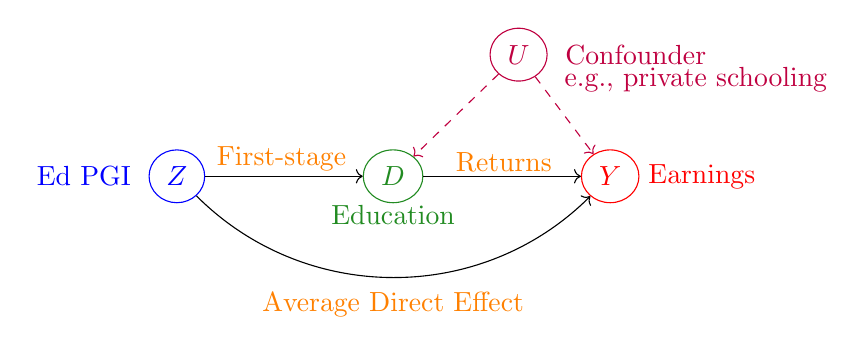
\begin{tikzpicture}
            % First nodes, Z, D, Y
            \node[state,ForestGreen] (treatment) at (0,0) {$D$};
            \node[state,blue] (instrument) [left=2cm of treatment] {$Z$};
            \path[->] (instrument) edge (treatment);
            % Labels for Z, D, Y
            \node[state,red] (outcome) [right=2cm of treatment] {$Y$};
            \node[color=blue] [left=0.1cm of instrument] {Ed PGI};
            \node[color=ForestGreen] [below=-0.1cm of treatment] (education) {Education};
            \node[text width=0.1cm, color=red] [right=-0.01cm of outcome] {Earnings};
            % Label the effects of interest.
            \node[text height=0.5cm, color=orange] [above left=-0.3cm and 0.2cm of treatment] {First-stage};
            \path[->] (treatment) edge (outcome);
            \node[text height=0.5cm, color=orange] [above right=-0.3 and 0.4cm of treatment] {Returns};
            \path[->] (instrument) edge[bend right=45] (outcome);
            \node[color=orange] [below=1cm of treatment] {Average Direct Effect};
            % Add on the unobserved confounder.
            \node[state,purple] (confounder) [above right=1.5cm of treatment] {$U$};
            \path[->,dashed,color=purple] (confounder) edge (treatment);
            \path[->,dashed,color=purple] (confounder) edge (outcome);
            \node[color=purple] [right=0.1cm of confounder] {Confounder};
            \node[color=purple] [below right=-0.2cm and 0.2cm of confounder] {e.g., private schooling};
        \end{tikzpicture}
    \end{figure}
    \vspace{-0.125cm}
    UKB has no info on private schooling\ldots
    \begin{itemize}
        \item \textcolor{red}{Selection bias} from not controlling for private schooling
        \item Overestimate education returns $\to$ biased direct $+$ indirect estimates.
    \end{itemize} 
\end{frame}
%-------------------------------------------------------------------------------
\begin{frame}
    \frametitle{Direct and Indirect Effects: Selection Bias}
    \textbf{Side-quest:}
    Why should we not use mediation methods off-the-shelf?
    \begin{figure}
        \makebox[\textwidth][c]{
            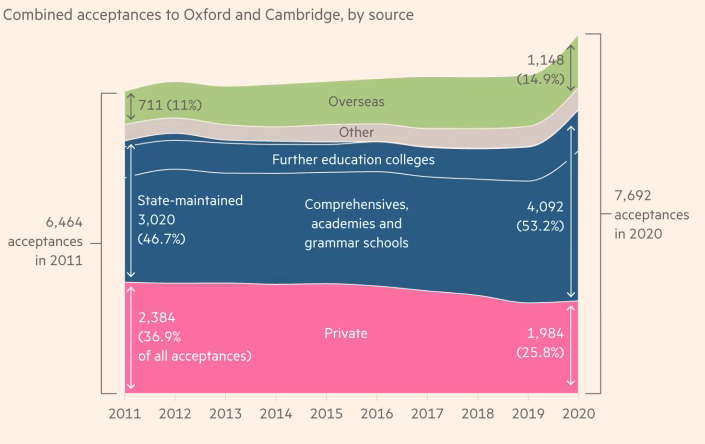
\includegraphics[width=0.6\textwidth]{
                presentation-files/headlines/oxford-private-2021.png}}
        \caption{$< 6$\% British children in private schools, but massively overrepresented at elite unis (FT, 2021).}
    \end{figure}
    \vspace{-0.125cm}
    UKB has no info on private schooling\ldots
    \begin{itemize}
        \item \textcolor{red}{Selection bias} from not controlling for private schooling
        \item Overestimate education returns $\to$ biased direct $+$ indirect estimates.
    \end{itemize} 
\end{frame}
%-------------------------------------------------------------------------------
\begin{frame}
    \frametitle{Direct and Indirect Effects: Selection Bias}
    \begin{itemize}
        \item \textcolor{red}{Selection bias} from not controlling for private education.
        \pause
        \item Motivates finding \textcolor{ForestGreen}{plausibly random education variation} in Britain, to avoid selection bias.
    \end{itemize}
    \vspace{-0.5cm}
    \begin{figure}
        \centering
        \singlespacing
        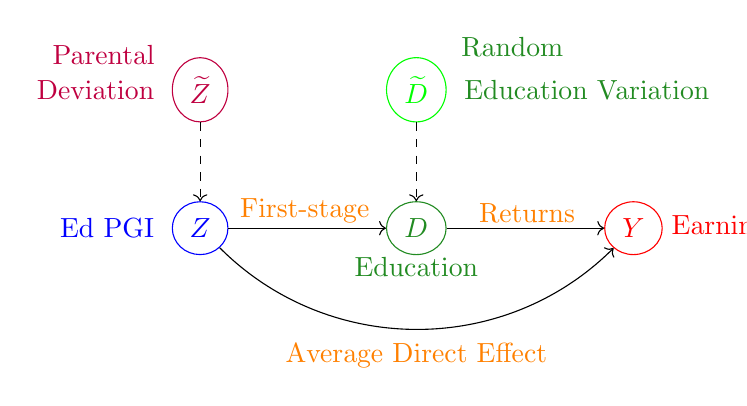
\begin{tikzpicture}
            % First nodes, Z, D, Y
            \node[state,ForestGreen] (treatment) at (0,0) {$D$};
            \node[state,blue] (instrument) [left=2cm of treatment] {$Z$};
            \path[->] (instrument) edge (treatment);
            % Labels for Z, D, Y
            \node[state,red] (outcome) [right=2cm of treatment] {$Y$};
            \node[color=blue] [left=0.1cm of instrument] {Ed PGI};
            \node[color=ForestGreen] [below=-0.1cm of treatment] (education) {Education};
            \node[text width=0.1cm, color=red] [right=-0.01cm of outcome] {Earnings};
            % Label the effects of interest.
            \node[text height=0.5cm, color=orange] [above left=-0.3cm and 0.2cm of treatment] {First-stage};
            \path[->] (treatment) edge (outcome);
            \node[text height=0.5cm, color=orange] [above right=-0.3 and 0.4cm of treatment] {Returns};
            \path[->] (instrument) edge[bend right=45] (outcome);
            \node[color=orange] [below=1cm of treatment] {Average Direct Effect};
            % Add on the overlapping research design
            % For Ed PGI
            \pause
            \node[state,purple] (instrument-instrument) [above=1cm of instrument] {$\tilde Z$};
            \path[->,dashed] (instrument-instrument) edge (instrument);
            \node[color=purple] [above left=-0.1cm and 0.2cm of instrument-instrument] {Parental};
            \node[color=purple] [left=0.1cm of instrument-instrument] {Deviation};
            % For Education
            \pause
            \node[state,green] (treatment-instrument) [above=1cm of treatment] {$\tilde D$};
            \path[->,dashed] (treatment-instrument) edge (treatment);
            % Label the overlapping instruments
            \node[color=ForestGreen] [above right=0.01cm and 0.175cm of treatment-instrument] {Random};
            \node[color=ForestGreen] [right=0.1cm of treatment-instrument] {Education Variation};
        \end{tikzpicture}
        \caption{Overlapping Research Design.}
    \end{figure}
    \vspace{-0.25cm}
    \[ \implies \text{Identifies average direct} + \text{indirect effects, local to } \tilde D \text{ compliers.} \]
\end{frame}
%-------------------------------------------------------------------------------
\begin{frame}[noframenumbering]
    \frametitle{Direct and Indirect Effects: Selection Bias}
    \begin{itemize}
        \item \textcolor{red}{Selection bias} from not controlling for private education.
        \pause
        \item Motivates finding \textcolor{ForestGreen}{plausibly random education variation} in Britain.
    \end{itemize}
    \vspace{-0.5cm}
    \begin{figure}[h!]
        \centering
        \singlespacing
        \begin{subfigure}[b]{0.575\textwidth}
            \centering
            \caption{Tuition Fees, Britain\\(Brookings, End of Free College in England, 2017).}
            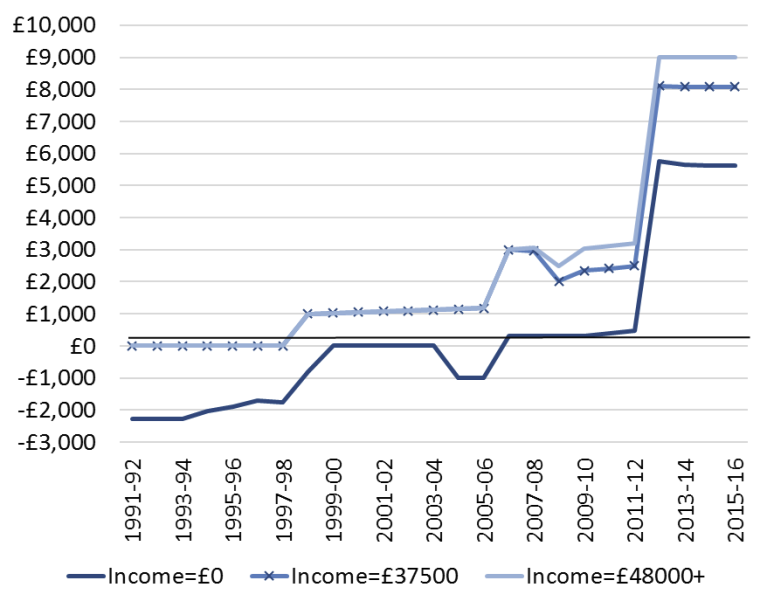
\includegraphics[width=\textwidth]{
                presentation-files/headlines/british-tuition-fees.png}
        \end{subfigure}
        \hfill
        \begin{subfigure}[b]{0.375\textwidth}
            \centering
            \caption{Changes in Mandatory School-Leaving Age, Britain.}
            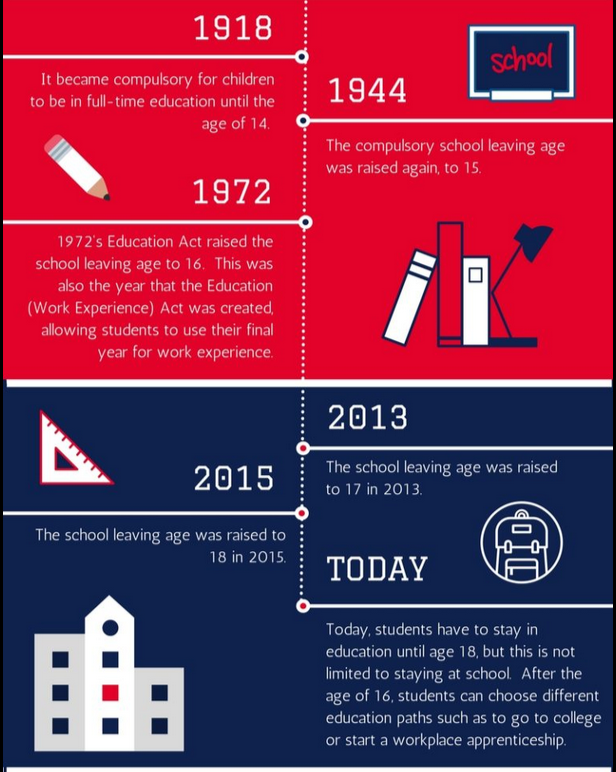
\includegraphics[width=\textwidth]{
                presentation-files/headlines/british-school-age.png}
        \end{subfigure}
    \end{figure}
\end{frame}
%-------------------------------------------------------------------------------
\subsection{(Optional) Correlational Results, HRS Data}
%-------------------------------------------------------------------------------
\begin{frame}
    \frametitle{(Optional) Correlational Results, HRS Data}
    Total Association:
    \vspace{-1.125cm}
    \begin{figure}
        \centering
        \singlespacing
        
\begin{tikzpicture}
            \node[state,blue] (instrument) at (0,0) {$Z$};
            \node[state,red] (outcome) [right=1.5cm of instrument] {$Y$};
            \path[->] (instrument) edge (outcome);
            % Label the nodes with econ examples
            \node[color=blue] [left=0.1cm of instrument] {Ed PGI};
            \node[text width=0.1cm, color=red] [right=-0.01cm of outcome] {Earnings};
        \end{tikzpicture}
    \end{figure}
    \vspace{-0.5cm}
    \begin{figure}
        \centering
        \caption{Bin Scatter Between \textcolor{blue}{Ed PGI}
            $+$ \textcolor{red}{Annual Earnings.}}
        \makebox[\textwidth][c]{
            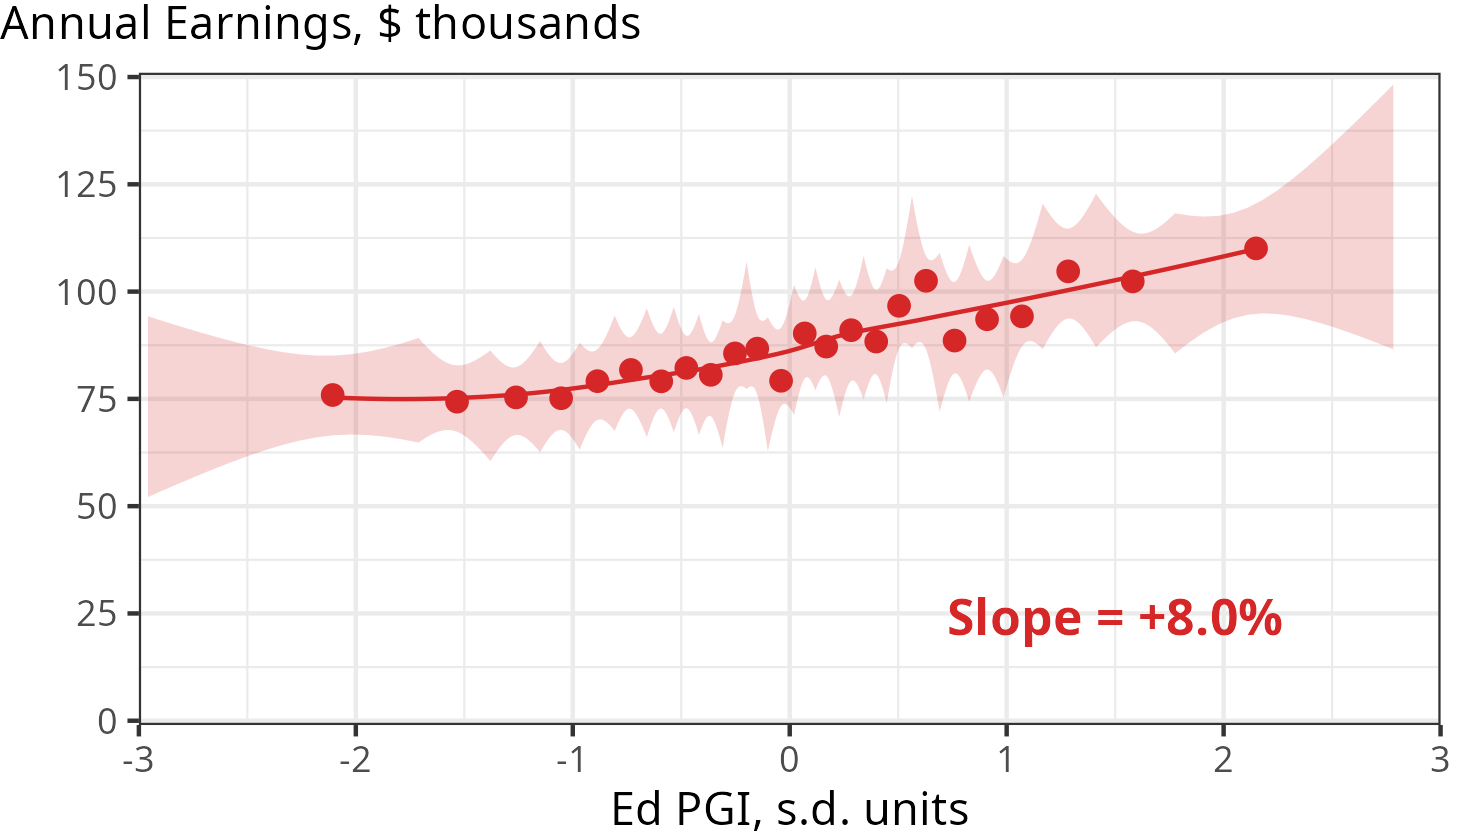
\includegraphics[width=0.8\textwidth]{
                ../text/sections/figures/genescore-earnings-wider}}
    \end{figure}
\end{frame}
%-------------------------------------------------------------------------------
\begin{frame}[noframenumbering]
    \frametitle{(Optional) Correlational Results, HRS Data}
    Total Association:
    \vspace{-1.125cm}
    \begin{figure}
        \centering
        \singlespacing
        
\begin{tikzpicture}
            \node[state,blue] (instrument) at (0,0) {$Z$};
            \node[state,red] (outcome) [right=1.5cm of instrument] {$Y$};
            \path[->] (instrument) edge (outcome);
            % Label the nodes with econ examples
            \node[color=blue] [left=0.1cm of instrument] {Ed PGI};
            \node[text width=0.1cm, color=red] [right=-0.01cm of outcome] {Earnings};
        \end{tikzpicture}
    \end{figure}
    \vspace{-0.5cm}
    \begin{figure}
        \centering
        \singlespacing
        \makebox[\textwidth][c]{
            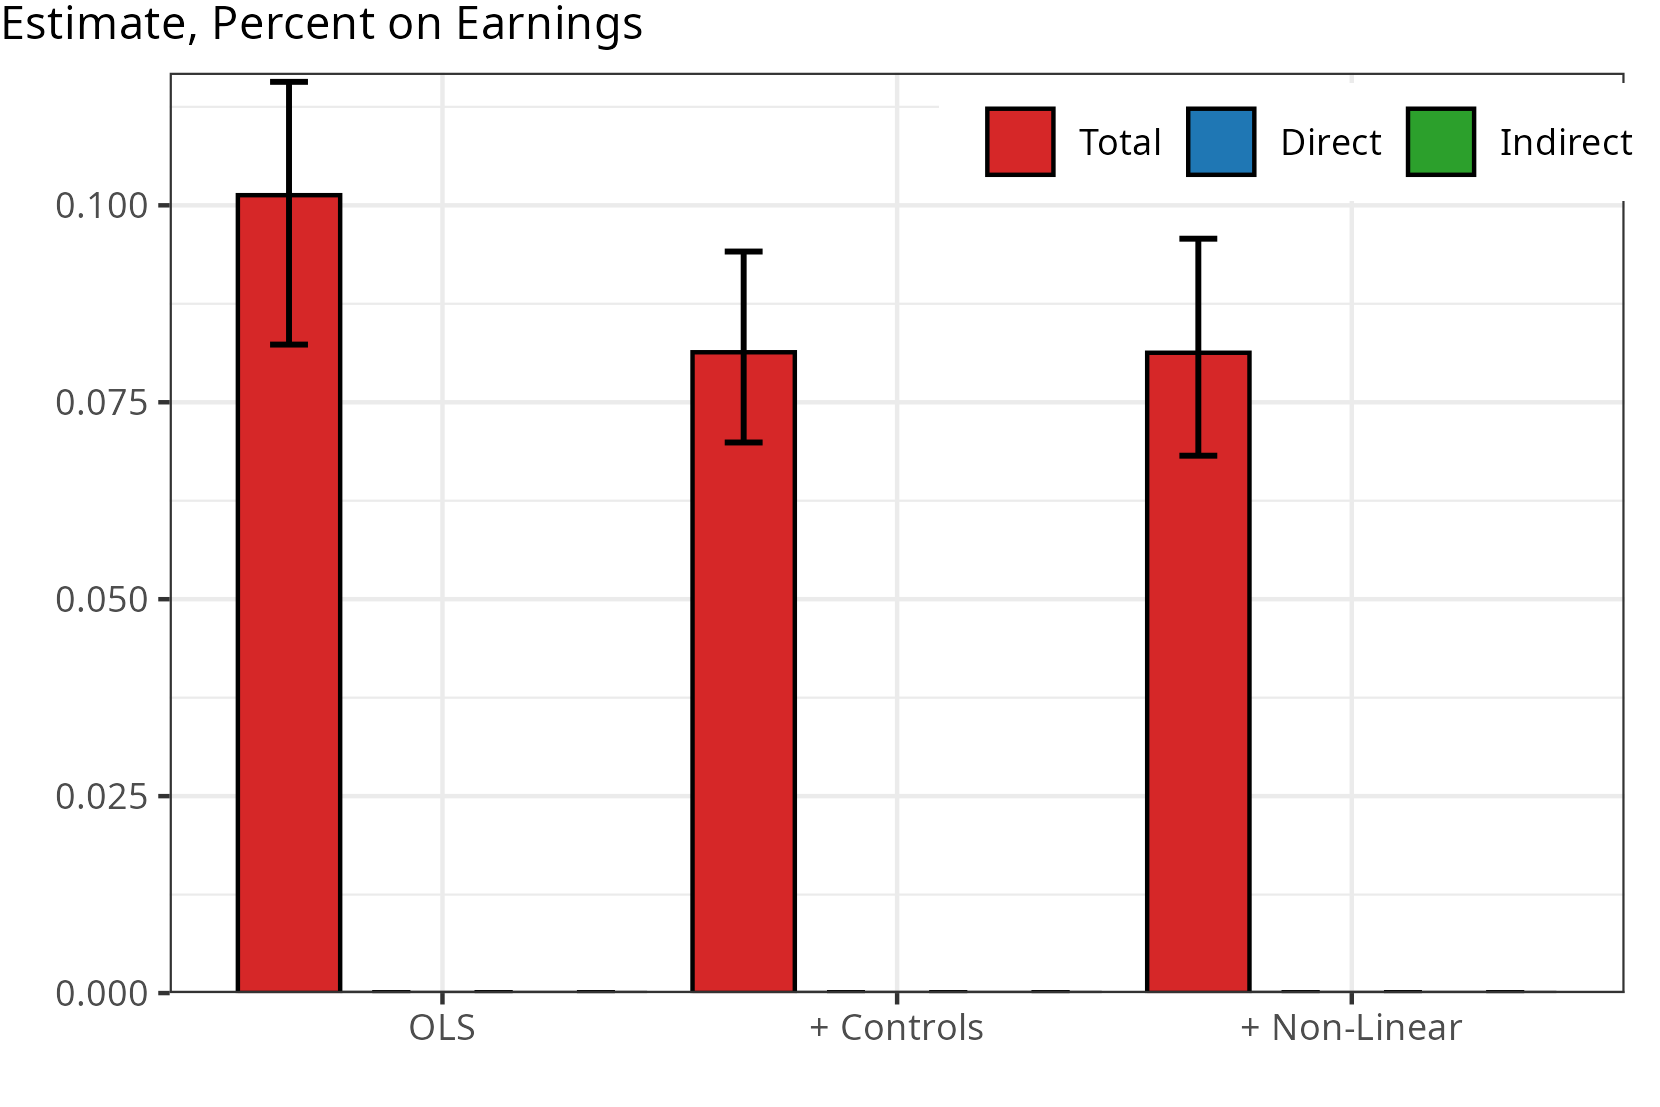
\includegraphics[width=0.9\textwidth]{
                ../text/sections/figures/mediation-total-plot.png}}
    \end{figure}
\end{frame}
%-------------------------------------------------------------------------------
\begin{frame}[noframenumbering]
    \frametitle{(Optional) Correlational Results, HRS Data}
    Decomposition:
    \vspace{-1.5cm}
    \begin{figure}
        %\centering
        \singlespacing
        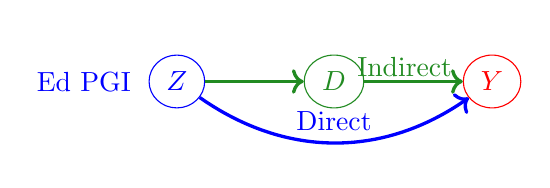
\begin{tikzpicture}
            \node[state,ForestGreen] (treatment) at (0,0) {$D$};
            \node[state,blue] (instrument) [left=1.25cm of treatment] {$Z$};
            \node[state,red] (outcome) [right=1.25cm of treatment] {$Y$};
            %\path[->] (instrument) edge (treatment);
            %\path[->] (treatment) edge (outcome);
            % Label the nodes with econ examples
            \node[color=blue] [left=0.1cm of instrument] {Ed PGI};
            \node[text height=0.5cm, color=ForestGreen] [above right=-0.3cm and -0.1cm of treatment] {Indirect};
            % Add in direct effects.
            %\path[->] (instrument) edge[bend right=45] (outcome);
            % Label the pathways with the colours
            \path[->, very thick, color=ForestGreen] (instrument) edge (treatment);
            \path[->, very thick, color=ForestGreen] (treatment) edge (outcome);
            \path[->, very thick, color=blue] (instrument) edge[bend right=35] (outcome);
            \node[text height=0.25cm, color=blue] [below=-0.1cm of treatment] {Direct};
        \end{tikzpicture}
    \end{figure}
    \vspace{-1cm}
    \begin{figure}
        \centering
        \singlespacing
        \makebox[\textwidth][c]{
            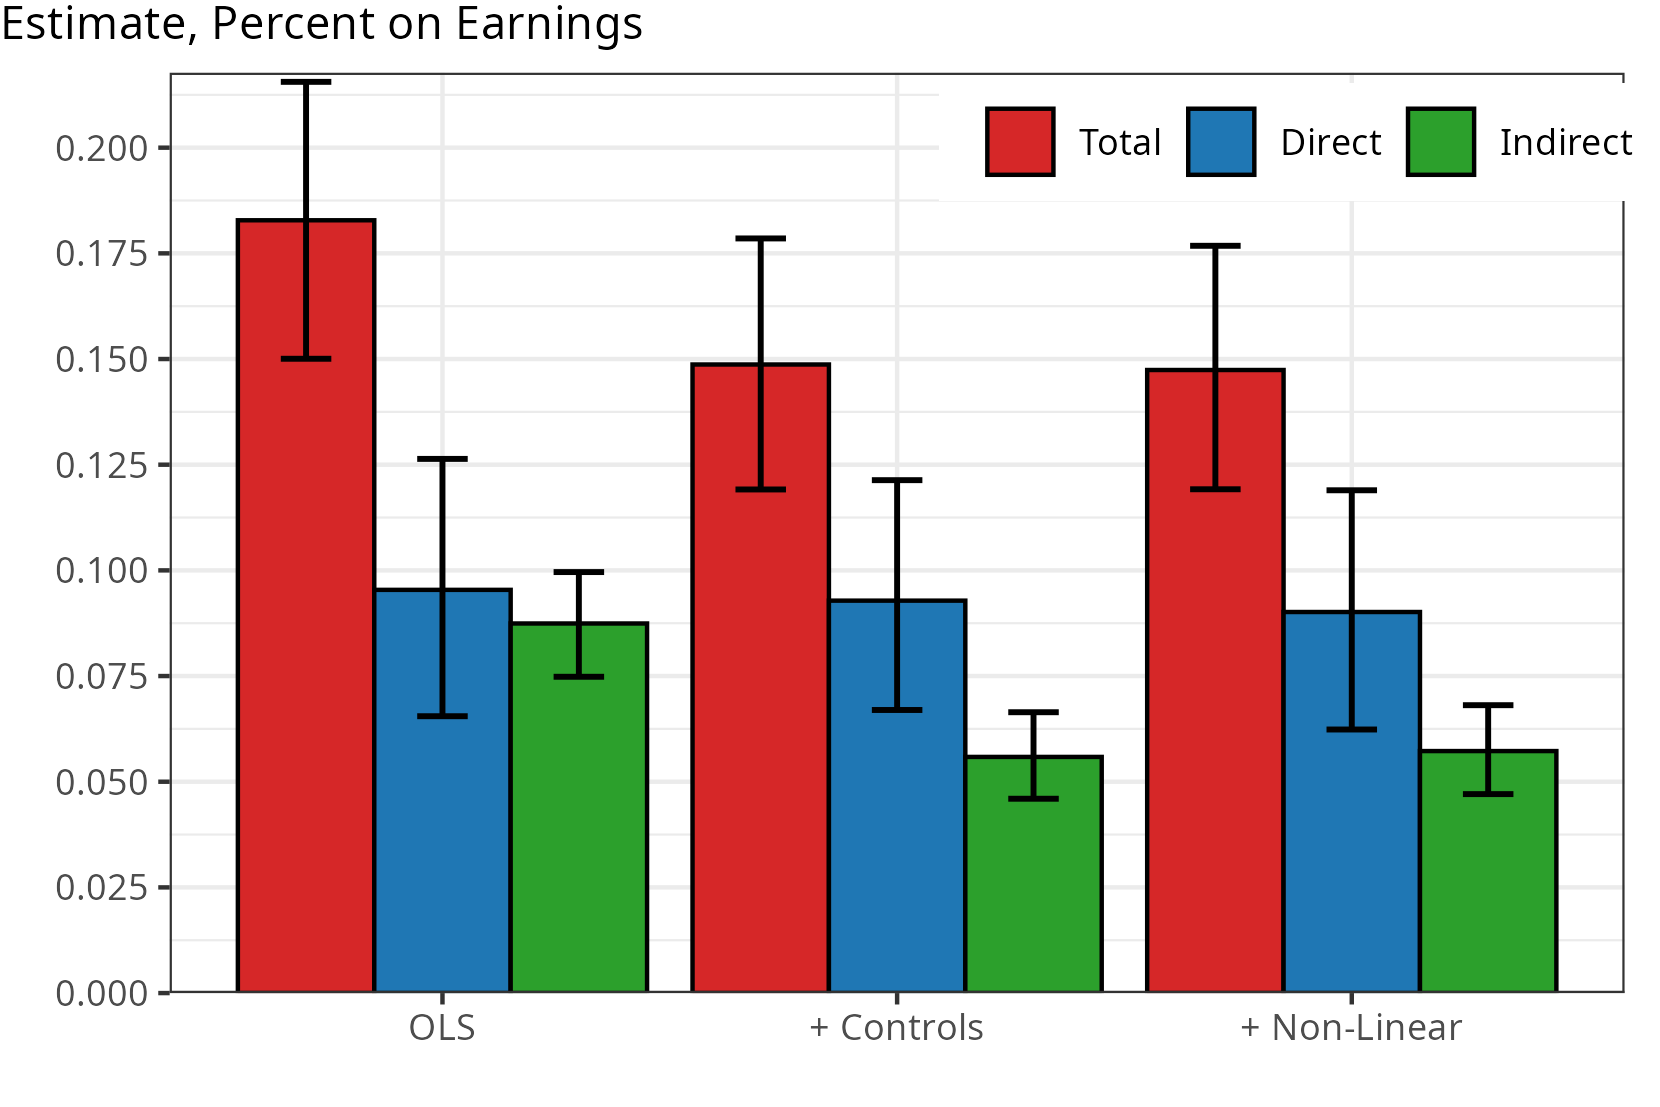
\includegraphics[width=0.9\textwidth]{
                ../text/sections/figures/mediation-plot.png}}
    \end{figure}
\end{frame}
%-------------------------------------------------------------------------------
\begin{frame}[noframenumbering]
    \frametitle{(Optional) Correlational Results, HRS Data}
    Percent through education:
    \vspace{-0.25cm}
    \begin{figure}
        \centering
        \singlespacing
        \makebox[\textwidth][c]{
            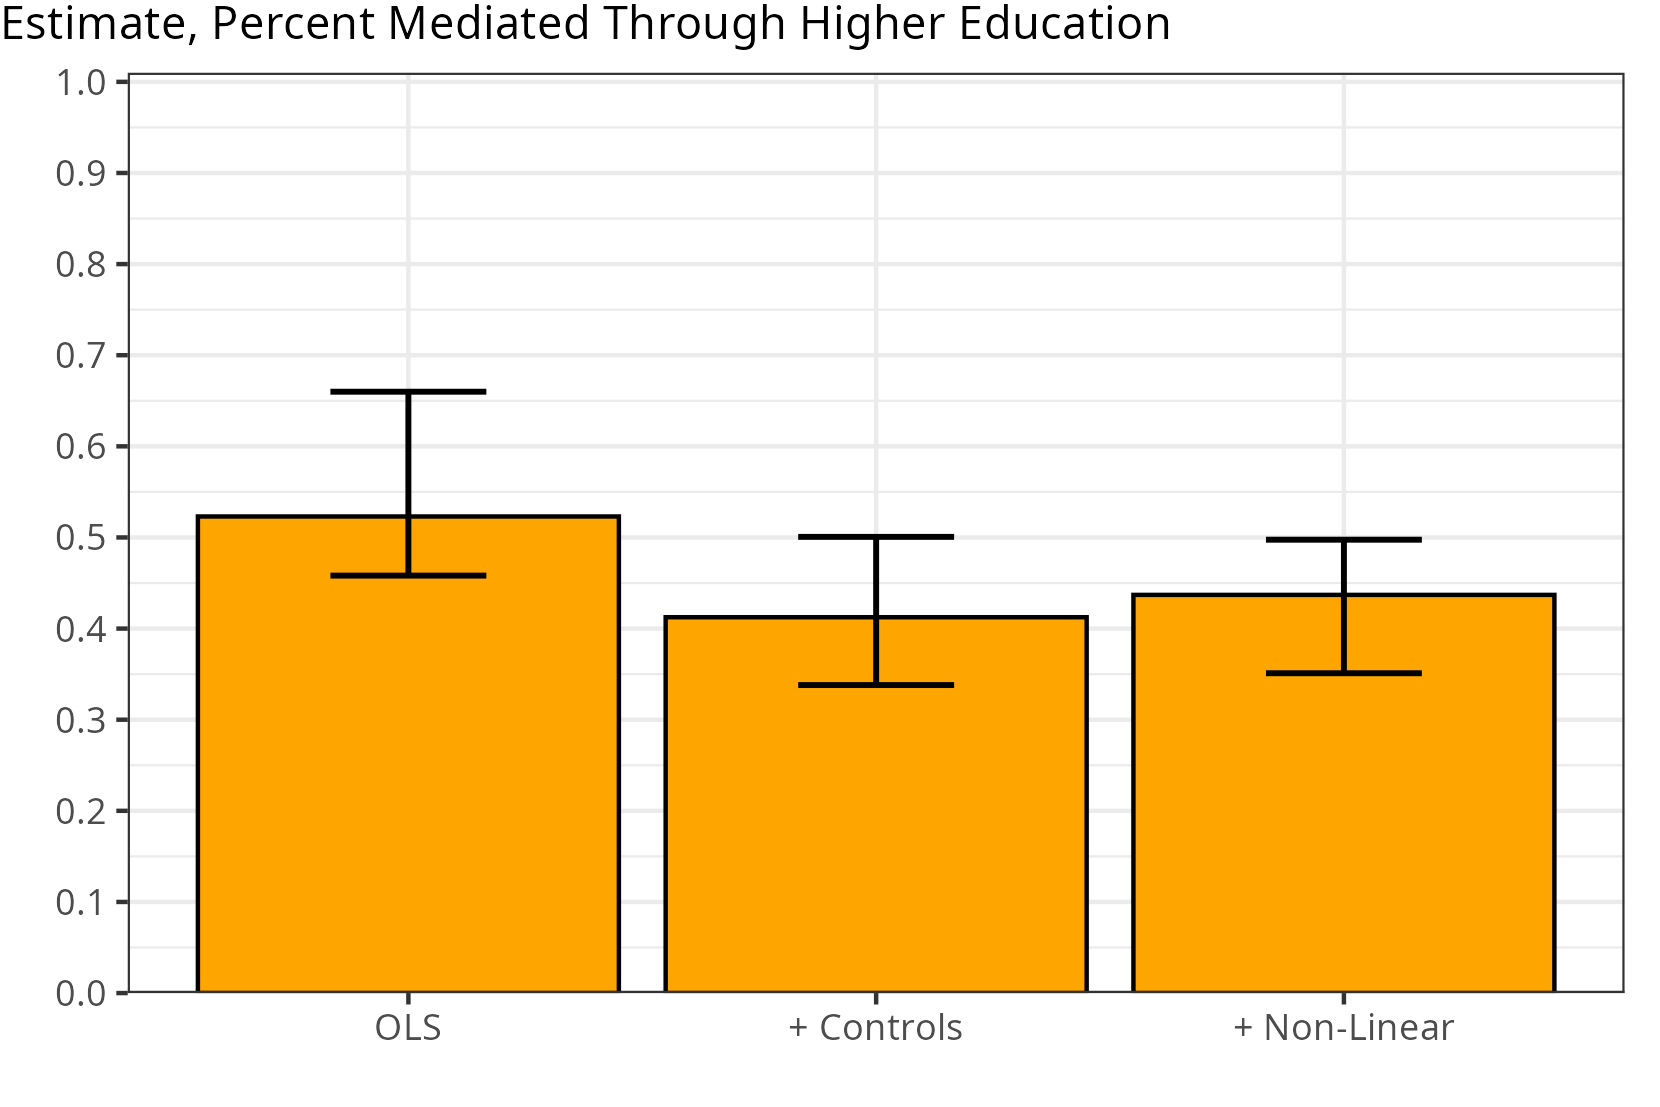
\includegraphics[width=0.9\textwidth]{
                ../text/sections/figures/mediation-percent-plot.png}}
    \end{figure}
\end{frame}
%-------------------------------------------------------------------------------
\begin{frame}
    \frametitle{(Optional) Correlational Results, HRS Data}
    Same results, with structural adjustment for selection into education:
    \vspace{-0.25cm}
    \begin{figure}
        \centering
        \singlespacing
        \makebox[\textwidth][c]{
            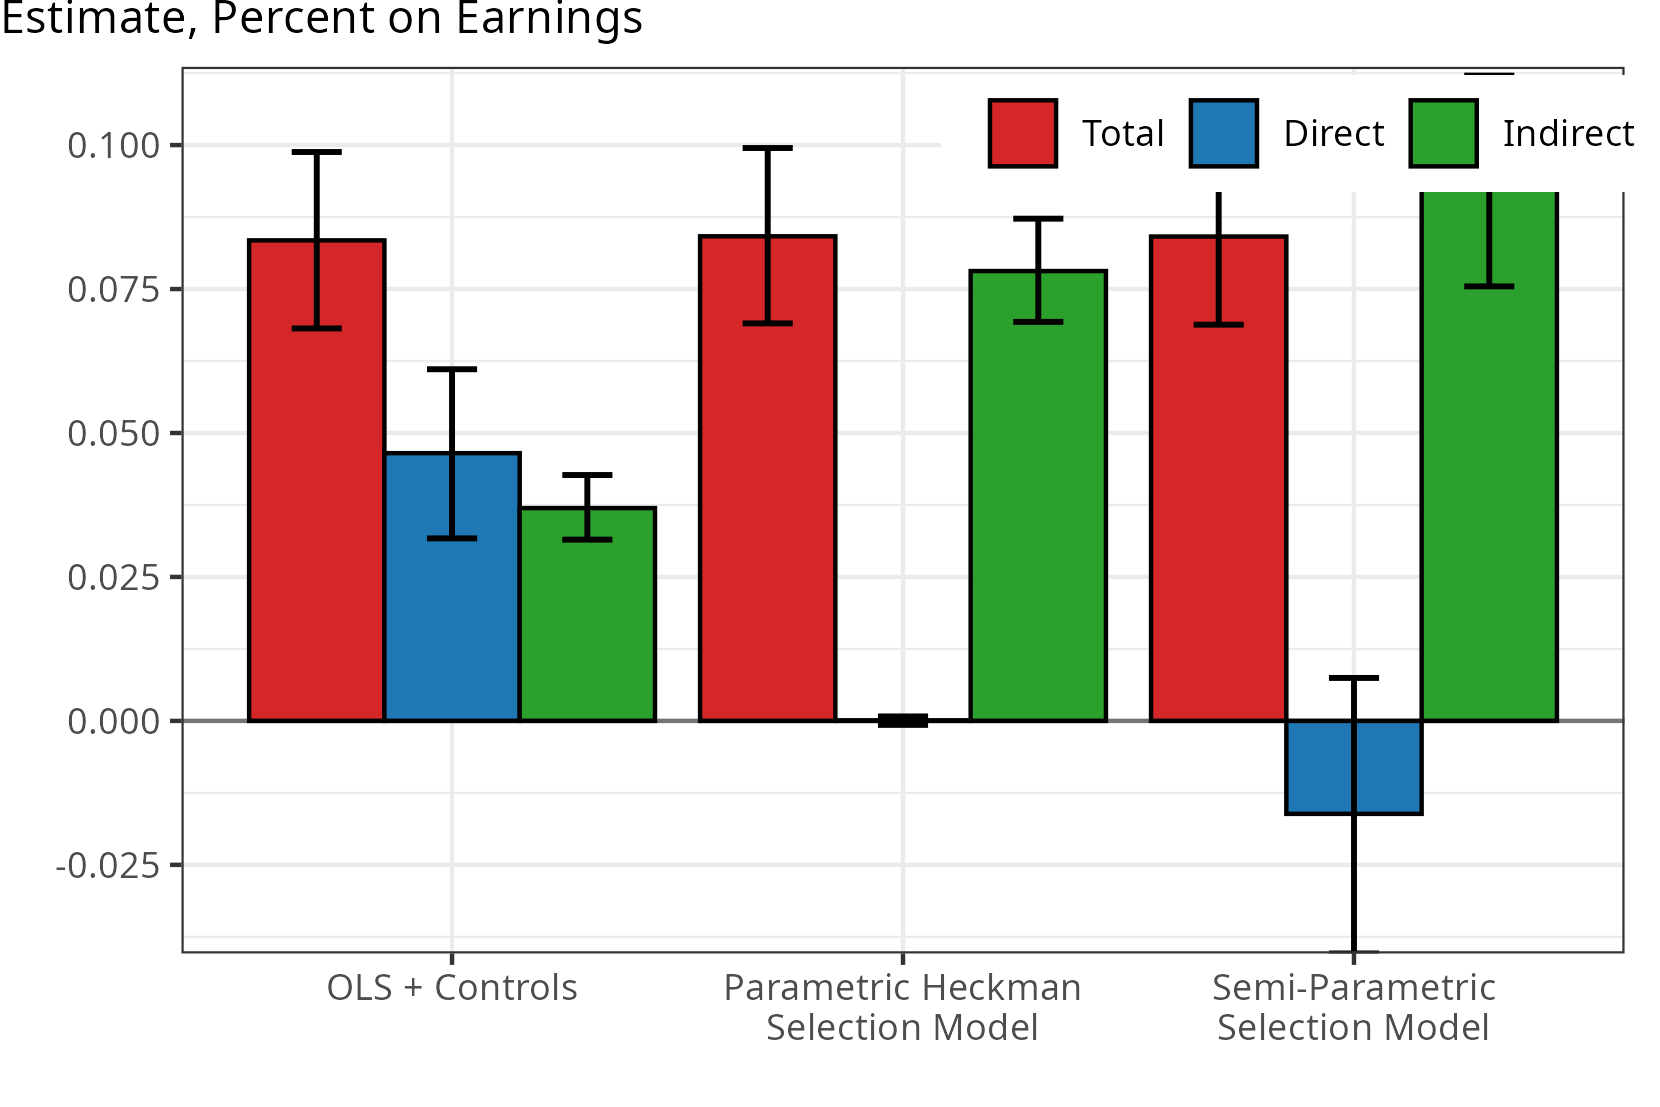
\includegraphics[width=0.9\textwidth]{
                ../text/sections/figures/mediation-selection-plot.png}}
    \end{figure}
    \vspace{-0.625cm}
    
    $\implies$ Returns to education unaffected, direct genetic channel $\to 0$. 
\end{frame}
%-------------------------------------------------------------------------------
\begin{frame}[noframenumbering]
    \frametitle{Direct and Indirect Effects}
    HRS Results with structural assumptions for identification:
    \vspace{-0.25cm}
    \begin{figure}
        \centering
        \singlespacing
        \makebox[\textwidth][c]{
            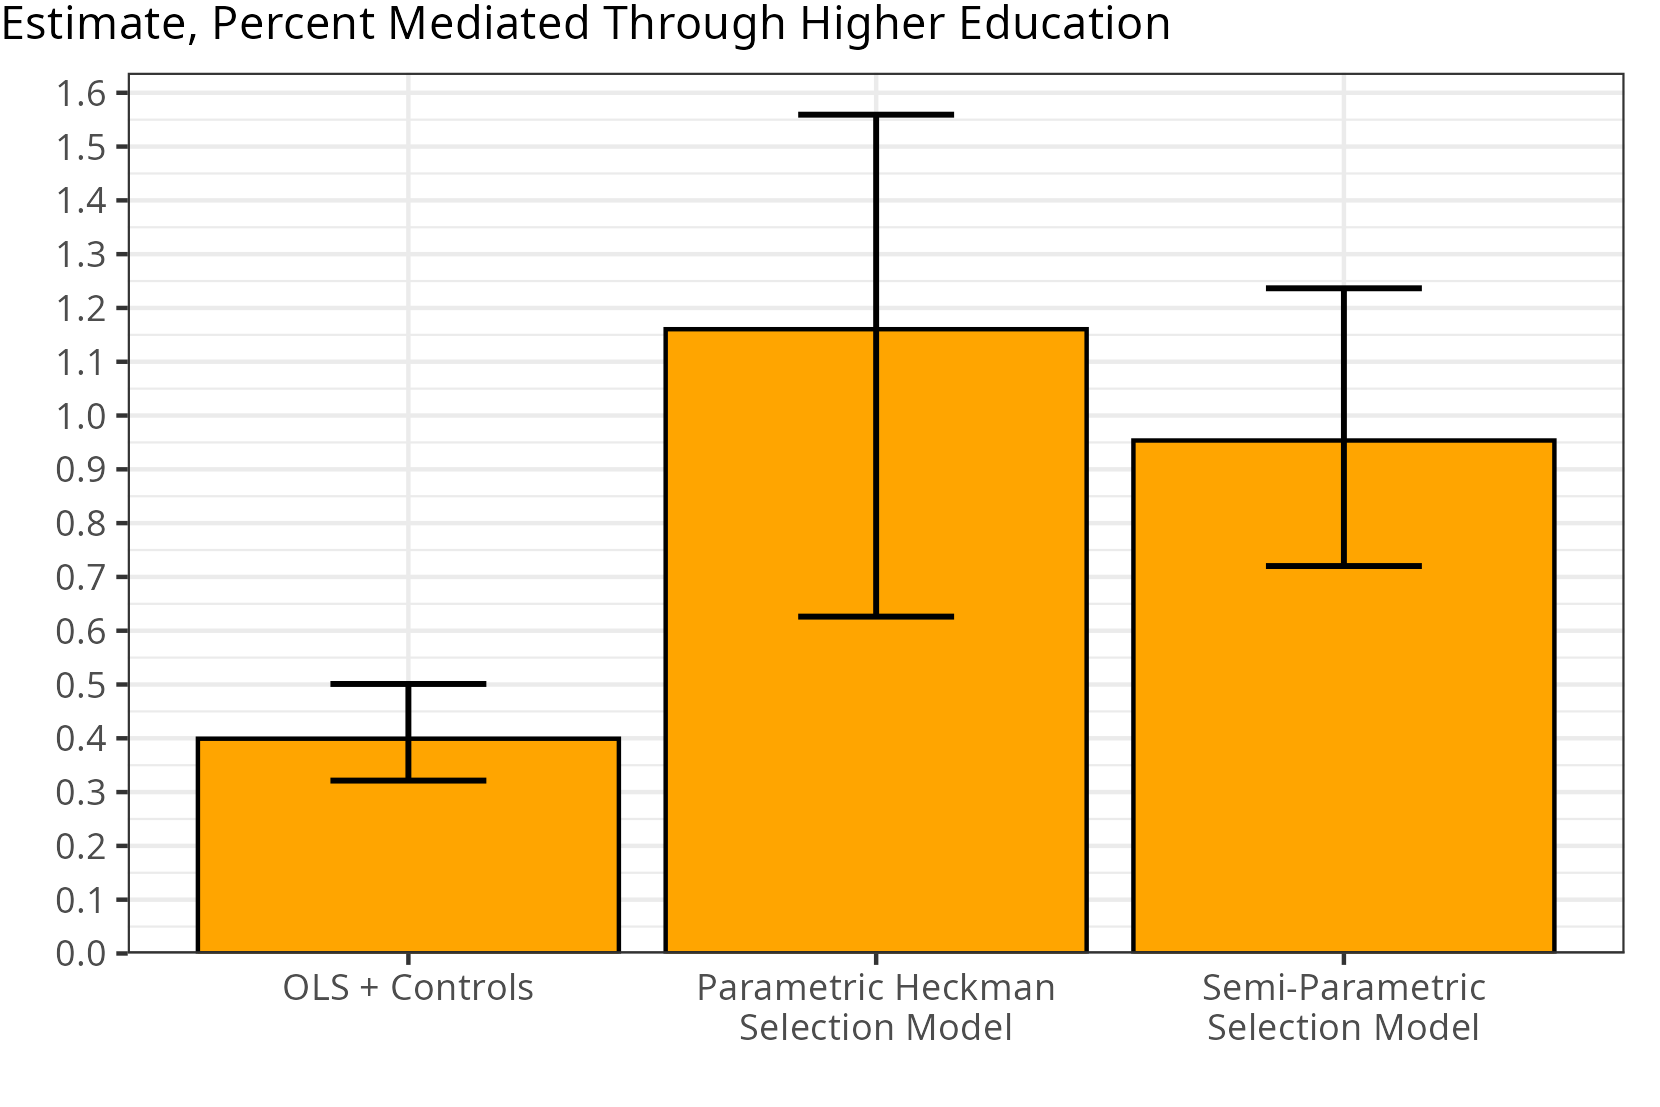
\includegraphics[width=0.9\textwidth]{
                ../text/sections/figures/mediation-selection-percent-plot.png}}
    \end{figure}
\end{frame}
%-------------------------------------------------------------------------------
\begin{frame}
    \frametitle{Conclusion}
    \begin{beamercolorbox}{postit}
        \raggedright
        \vspace{0.01cm} \\
        ``\textbf{The difference of natural talents in different men}, is, in reality, much less than we are aware of [\ldots].
        The difference between the most dissimilar characters, between a philosopher and a common street porter, seems to arise \textbf{not so much from nature, as from habit, custom, and education}.''
        \hfill
        \underline{\textit{Adam Smith (1776), The Wealth of Nations, Volume 1 p. 16.}}
        \vspace{0.02cm}
    \end{beamercolorbox}
    \vspace{0.25cm}
    
    \textbf{This Project:}
    \begin{enumerate}
        \item Studies total genetic effects, on later-life labour outcomes (earnings).
        \item Design-based decomposition, effect of \textcolor{red}{Ed PGI $\to$ Earnings} to \textcolor{blue}{direct (genetic)} $+$ \textcolor{ForestGreen}{indirect (education)} effects.
        \item Overlapping research design for causal effects (UK Biobank), in-progress.
    \end{enumerate}
    \vfill

    \hrulefill
    
    Thank you for your listening to my presentation.
    \vspace{0.25cm}
    
    Comments welcome now, later, or at \href{mailto:seh325@cornell.edu}{\textcolor{blue}{seh325@cornell.edu}}.
    %\begin{beamercolorbox}{postit}
    %    \small
    %    \vspace{0.025cm}
    %    
    %    %\raggedright
    %    ``The evidence suggests \textbf{fluid intelligence and self-control partly mediate} the relationship between the Ed PGI and education.''
    %    
    %    \underline{\textit{Abstract --- Carvalho (2024, JPE Micro)}}
    %    \vspace{0.025cm}
    %\end{beamercolorbox}
\end{frame}
%-------------------------------------------------------------------------------
\begin{frame}[noframenumbering]
    \frametitle{Appendix: Mediation Equations}
    \label{mediation-equations}
    Mediation methods decompose the total effect to direct $+$ indirect channels.
    E.g., OLS simultaneous regression (Imai Keele Yamamoto, 2010):\footnote[frame]{
        Usually estimated with added controls, $+ \vec \zeta' \vec X_i$.
    }
    \begin{align*}
        &\textcolor{blue}{Z_i \leftarrow \text{ Ed PGI}} &
        \text{First-stage: }
            \textcolor{ForestGreen}{D_i}
                &= \phi + \pi \textcolor{blue}{Z_i} + \eta_i \\
        &\textcolor{ForestGreen}{D_i \leftarrow \text{ Education years}} &
        \text{Second-stage: }
            \textcolor{red}{Y_i}
                &= \alpha
                    + \beta \textcolor{ForestGreen}{D_i}
                    + \gamma \textcolor{blue}{Z_i}
                    + \delta \textcolor{blue}{Z_i} \textcolor{ForestGreen}{D_i}
                    + \varepsilon_i \\
        &\textcolor{red}{Y_i \leftarrow \text{ log(Earnings)}} &
            \implies \textcolor{Orange}{\text{Direct Effect }}
            &= \gamma + \delta \E{\textcolor{ForestGreen}{D_i}} \\
        &   &\textcolor{Orange}{\text{Indirect Effect }}
            &= \pi \left( \beta + \delta \E{\textcolor{blue}{Z_i}} \right)
    \end{align*}

    i.e., a regression decomposition, asumming \\
    (1) seq ignorablility, (2) linear outcome model, (3) homogenous TEs:
    \vspace{-0.5cm}
    \begin{figure}
        \centering
        \singlespacing
        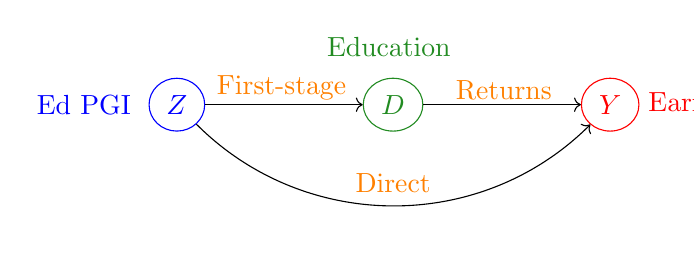
\begin{tikzpicture}
            \node[state,ForestGreen] (treatment) at (0,0) {$D$};
            \node[state,blue] (instrument) [left=2cm of treatment] {$Z$};
            \path[->] (instrument) edge (treatment);
            \node[color=blue] [left=0.1cm of instrument] {Ed PGI};
            \node[text width=1.675cm, color=ForestGreen] [above=0.15cm of treatment] (education) {Education};
            \node[color=orange] [above left=-0.3cm and 0.2cm of treatment] {First-stage};
            \node[state,red] (outcome) [right=2cm of treatment] {$Y$};
            \path[->] (treatment) edge (outcome);
            \node[text width=0.1cm, color=red] [right=-0.01cm of outcome] {Earnings};
            \node[text height=0.5cm, color=orange] [above right=-0.3 and 0.4cm of treatment] {Returns};
            % Add in direct effects.
            \path[->] (instrument) edge[bend right=45] (outcome);
            \node[text height=0.25cm, color=orange] [below=0.4cm of treatment] {Direct};
        \end{tikzpicture}
    \end{figure}
\end{frame}
%-------------------------------------------------------------------------------
\begin{frame}[noframenumbering]
    \frametitle{Appendix: Bias in Direct Effect Estimates}
    \label{selection-bias-equations}
    \vspace{-0.5cm}
    \[ \text{\textcolor{purple}{Estimand, Direct}}
        = \text{\textcolor{blue}{Direct Effect}}
            + \Big(\text{\textcolor{red}{Selection Bias}}
            + \text{\textcolor{orange}{Complier Bias}}\Big) \]
    \vspace{-0.25cm}
    \begin{align*}
        & \underbrace{\mathbb E_{D_i} \Big[
            \Egiven{Y_i}{Z_i = 1, D_i} - \Egiven{Y_i}{Z_i = 0, D_i} \Big]}_{
                \text{\textcolor{purple}{Estimand, Direct Effect}} } \\
        & = \underbrace{\E{Y_i(1, D_i(Z_i)) - Y_i(0, D_i(Z_i))}}_{
            \text{\textcolor{blue}{Average Direct Effect}}} \\
        & \;\;\;\; + \underbrace{ \mathbb E_{D_i} \Big[ 
            \Egiven{Y_i(0, D_i(Z_i))}{D_i(1) = d} 
            - \Egiven{Y_i(0, D_i(Z_i))}{D_i(0) = d} \Big] }_{
                \text{\textcolor{red}{Selection Bias}}} \\
        & \;\;\;\; + \underbrace{ \E[D_i ]{
            \begin{aligned}
            &\Big(1 - \Prob{D_i(1) = d} \Big) \\
            &\times \left( \begin{aligned}
                &\Egiven{Y_i(1, D_i(Z_i)) - Y_i(0, D_i(Z_i))}{D_i(1) = d} \\ 
                &  - \Egiven{Y_i(1, D_i(Z_i)) - Y_i(0, D_i(Z_i))}{D_i(0) = 1- d}
                \end{aligned} \right) \end{aligned}} }_{
                    \text{\textcolor{orange}{Complier Bias}}}
    \end{align*}
\end{frame}
%-------------------------------------------------------------------------------
\begin{frame}[noframenumbering]
    \frametitle{Appendix: Bias in Indirect Effect Estimates}
    \vspace{-0.5cm}
    \[ \text{\textcolor{purple}{Estimand, Indirect}}
        = \text{\textcolor{ForestGreen}{Indirect Effect}}
            + \Big(\text{\textcolor{red}{Selection Bias}}
            + \text{\textcolor{orange}{Non-complier Bias}}\Big) \]
    \vspace{-0.25cm}
    \small
    \begin{align*}
        & \underbrace{\E[Z_i]{
            \Big( \Egiven{D_i}{Z_i = 1} - \Egiven{D_i}{Z_i = 0} \Big) \times
            \Big( \Egiven{Y_i}{Z_i, D_i = 1} - \Egiven{Y_i}{Z_i, D_i = 0} \Big) }}_{ \text{\textcolor{purple}{Estimand, Indirect Effect}} } \\
        & = \underbrace{\E{Y_i(Z_i, D_i(1)) - Y_i(Z_i, D_i(0))}}_{
            \text{\textcolor{ForestGreen}{Indirect Effect}} } \\
        & \;\;\;\; + \underbrace{\Prob{D_i(1) = 1, D_i(0) = 0}  \Big(
            \Egiven{Y_i(Z_i, 0)}{D_i = 1} - \Egiven{Y_i(Z_i, 0)}{D_i = 0} \Big)}_{
                \text{\textcolor{red}{Selection Bias}}} \\
        & \;\;\;\; + \Prob{D_i(1) = 1, D_i(0) = 0} \times \\
        & \;\;\;\; \;\; \underbrace{ \left[ \begin{aligned}
            &\Big( 1 - \Prob{D_i=1} \Big)
            \left( \begin{aligned}
                &\Egiven{Y_i(Z_i, 1) - Y_i(Z_i, 0)}{D_i = 1} \\ 
                &  - \Egiven{Y_i(Z_i, 1) - Y_i(Z_i, 0)}{D_i = 0}
            \end{aligned} \right) \\
            &+ \left( \frac{1 - \Prob{D_i(1) = 1, D_i(0) = 0} }{
                \Prob{D_i(1) = 1, D_i(0) = 0}} \right)
            \left( \begin{aligned}
                &\Egiven{Y_i(Z_i, 1) - Y_i(Z_i, 0)}{D_i(1) = 0 \text{ or } D_i(0)=1} \\ 
                &  - \E{Y_i(Z_i, 1) - Y_i(Z_i, 0)}
            \end{aligned} \right)
        \end{aligned} \right]}_{\text{\textcolor{orange}{Non-complier Bias}}}
    \end{align*}
\end{frame}
%-------------------------------------------------------------------------------
\end{document}
